%%%%%%%%%%%%%%%%%%%%%%%%%%%%%%%%%%%%%%%%%
% The Legrand Orange Book
% LaTeX Template
% Version 2.4 (26/09/2018)
%
% This template was downloaded from:
% http://www.LaTeXTemplates.com
%
% Original author:
% Mathias Legrand (legrand.mathias@gmail.com) with modifications by:
% Vel (vel@latextemplates.com)
%
% License:
% CC BY-NC-SA 3.0 (http://creativecommons.org/licenses/by-nc-sa/3.0/)
%
% Compiling this template:
% This template uses biber for its bibliography and makeindex for its index.
% When you first open the template, compile it from the command line with the 
% commands below to make sure your LaTeX distribution is configured correctly:
%
% 1) pdflatex ponteiros_em_c
% 2) makeindex main.idx -s StyleInd.ist
% 3) biber main
% 4) pdflatex main x 2
%
% After this, when you wish to update the bibliography/index use the appropriate
% command above and make sure to compile with pdflatex several times 
% afterwards to propagate your changes to the document.
%
% This template also uses a number of packages which may need to be
% updated to the newest versions for the template to compile. It is strongly
% recommended you update your LaTeX distribution if you have any
% compilation errors.
%
% Important note:
% Chapter heading images should have a 2:1 width:height ratio,
% e.g. 920px width and 460px height.
%
%%%%%%%%%%%%%%%%%%%%%%%%%%%%%%%%%%%%%%%%%

%----------------------------------------------------------------------------------------
%	PACKAGES AND OTHER DOCUMENT CONFIGURATIONS
%----------------------------------------------------------------------------------------

\documentclass[11pt,fleqn]{book} % Default font size and left-justified equations

\input{structure.tex} % Insert the commands.tex file which contains the majority of the structure behind the template

%\hypersetup{pdftitle={Title},pdfauthor={Author}} % Uncomment and fill out to include PDF metadata for the author and title of the book

%----------------------------------------------------------------------------------------
%\includexmp{metadata}
\begin{document}
\renewcommand{\lstlistingname}{Programa}% Listing -> Programa

%----------------------------------------------------------------------------------------
%	TITLE PAGE
%----------------------------------------------------------------------------------------

\begingroup
\thispagestyle{empty} % Suppress headers and footers on the title page
\begin{tikzpicture}[remember picture,overlay]
\node[inner sep=0pt] (background) at (current page.center) {\includegraphics[width=\paperwidth]{background.png}};
\draw (current page.north) node [fill=ocre!30!white,fill opacity=0.6,text opacity=1,inner sep=1cm] at (6.8,-5){\Huge\centering\bfseries\sffamily\parbox[c][][t]{\paperwidth}{\centering Ponteiros e Arrays em C\\[15pt] % Book title
{\Large Tutorial definitivo}\\[20pt] % Subtitle
{\huge Texto Original: Ted Jensen\\ Adaptação/atualização: João Araujo}}}; % Author name
\end{tikzpicture}
\vfill
\endgroup

%----------------------------------------------------------------------------------------
%	COPYRIGHT PAGE
%----------------------------------------------------------------------------------------

\newpage
~\vfill
\thispagestyle{empty}

\doclicenseThis

\noindent CC BY-SA \copyright\ 2021\\ % Copyright notice

\noindent \textsc{Publicado por João Araujo}\\ % Publisher

\noindent \textsc{www.araujo.eng.uerj.br}\\ % URL

\noindent Licenciado pela Creative Commons Atribuição-CompartilhaIgual
CC BY-SA 4.0). Você não pode usar este arquivo, exceto em conformidade com a Licença. Você pode obter uma cópia da Licença em \url{https://creativecommons.org/licenses/by-sa/4.0/deed.pt_BR}. 

\noindent \textit{Primeira versão, Outubro de 2021} % Printing/edition date

%\noindent \textit{First printing, March 2019} % Printing/edition date

%----------------------------------------------------------------------------------------
%	TABLE OF CONTENTS
%----------------------------------------------------------------------------------------

%\usechapterimagefalse % If you don't want to include a chapter image, use this to toggle images off - it can be enabled later with \usechapterimagetrue

\chapterimage{candle-factory} % Table of contents heading image

\pagestyle{empty} % Disable headers and footers for the following pages

\tableofcontents % Print the table of contents itself

\cleardoublepage % Forces the first chapter to start on an odd page so it's on the right side of the book

\pagestyle{fancy} % Enable headers and footers again

%----------------------------------------------------------------------------------------
%	PART
%----------------------------------------------------------------------------------------

%\part{Part One}

%----------------------------------------------------------------------------------------
%	CHAPTER 1
%----------------------------------------------------------------------------------------

\chapterimage{beaumont-machine} % Chapter heading image

\chapter*{Prefácio}
Este texto nasceu da necessidade de ensinar ponteiros em C. O tópico de ponteiros sempre foi o grande terror de estudantes iniciais da linguagem de programação C e este tema não era bem esclarecido nos principais livros disponíveis. Apesar do medo dos estudantes, o tema não é complexo, mas exige muita atenção e uma compreensão muito boa sobre o hardware e como funcionam os computadores.

Sempre pensei em escrever um texto como esse, mas esta tarefa sempre foi deixada para depois, até que me deparei com o excelente texto de \textbf{Ted Jensen}. Felizmente ele colocou o texto em domínio público e assim pude aproveitá-lo sem restrições. No início seria apenas uma tradução, porém a última revisão deste texto foi feita há mais de 20 anos. Na época que Ted escreveu este livro e o disponibilizou gratuitamente, a licença \textit{Creative Commons }estava iniciando. Assim, em vez de distribuir como domínio público, escolhi distribuí-la com uma licença mais moderna que mantém o material disponível para todos e pede apenas uma declaração de atribuição.

Livros excelentes se perdem por questões de copyright. Os autores perdem o interesse no tema (ou coisa pior) e bons textos não podem ser atualizados para aproveitar os avanços na computação.

Antes de disponibilizá-lo tentei contato com Ted, mas todas as tentativas foram infrutíferas. O site original não funciona mais e o e-mail não responde. A última atualização do site foi em 2003 e em 2018 ele saiu do ar.

De qualquer modo, mesmo sem conseguir contactá-lo, deixo aqui meu profundo agradecimento a Ted pela sua generosidade em distribuir material de alta qualidade. A maior parte do texto aqui apresentado é minha tradução do texto original de Ted.

Fiz algumas adaptações para modernizar o texto. Na primeira versão do livro existia apenas o C ANSI, depois tivemos algumas pequenas modificações na linguagem que tentei incorporar ao texto original de Ted. 

Chegou um momento que deixou de ser apenas uma tradução, mas uma co-autoria, mas mantenho a gratuidade do texto para todos que queiram utilizá-lo. Assim, se você quiser usar este texto, peço apenas a citação deste material

O arquivo fonte em Latex deste texto pode ser obtido em\\ \url{https://github.com/jaraujouerj/Ponteiros-em-C}\\
e o arquivo em pdf pode ser baixado do meu site pessoal:\\
\url{http://araujo.eng.uerj.br}

\section*{Sobre mim}
Meu nome é João Araujo e sou professor do Departamento de Engenharia de Sistemas e Computação da Faculdade de Engenharia da Universidade do Estado do Rio de Janeiro desde 1990. Trabalho há anos ensinando programação principalmente com a linguagem C. Aprendi C ainda estudante, na UFRJ, nos anos 1980, na versão original do livro K\&R e acompanhei a transição de C por todas as suas versões: ANSI, C99 e C11.

\section*{Uso deste Material}
Tudo aqui contido é liberado sob a licença Creative Commons CC-by-SA. Qualquer pessoa pode copiar ou distribuir este material livremente, desde que siga os parâmetros desta licença. Assim como Ted, `\textit{`a única coisa que peço é que se este material for usado como um auxiliar de ensino em uma aula, eu agradeceria se fosse distribuído na íntegra, ou seja, incluindo todos os capítulos, o prefácio e a introdução. Eu também agradeceria se, em tais circunstâncias, o instrutor de tal classe me deixasse uma nota em um dos endereços abaixo informando-me sobre isso. Escrevi isso com a esperança de que seja útil a outras pessoas e, como não estou pedindo nenhuma remuneração financeira, a única maneira de saber que atingi, pelo menos parcialmente, esse objetivo é por meio do feedback de quem considera este material útil.}'

Instrutor ou não, se este material foi útil para você, me envie uma mensagem em \href{mailto:araujo@eng.uerj.br}{araujo@eng.uerj.br}. Críticas, correções e sugestões também são bem-vindas.

\begin{verbatim}
João Araujo Ribeiro
Departamento de Engenahria de Sistemas e Computação
Faculdade de Engenharia
Universidade do Estado do Rio de Janeiro
Outubro de 2021
\end{verbatim}

\section*{Prefácio original de Ted Jensen}
Este documento tem como objetivo apresentar dicas para programadores iniciantes na linguagem de programação C. Ao longo de vários anos lendo e contribuindo para várias conferências sobre C, incluindo as da \textit{FidoNet} e \textit{UseNet}, observei que um grande número de novatos em C parece ter dificuldade em compreender os fundamentos dos ponteiros. Portanto, empreendi a tarefa de tentar explicá-los em linguagem simples, com muitos exemplos.

A primeira versão deste documento foi colocada em domínio público. Ele foi escolhido por \textit{Bob Stout}, que o incluiu como um arquivo chamado \textbf{PTR-HELP.TXT} em sua coleção amplamente distribuída de \textbf{SNIPPETS}. Desde aquele lançamento original de 1995, adicionei uma quantidade significativa de material e fiz algumas pequenas correções no trabalho original.

Posteriormente, postei uma versão HTML por volta de 1998 em meu site em:\\
http://pweb.netcom.com/~tjensen/ptr/cpoint.htm

Depois de inúmeros pedidos, finalmente saí com esta versão em PDF que é idêntica à versão em HTML citada acima e que pode ser obtida no mesmo site.

\section*{Agradecimentos}
Há tantas pessoas que, sem saber, contribuíram para este trabalho por causa das perguntas que colocaram no \textit{FidoNet C Echo}, ou no \textit{UseNet Newsgroup comp.lang.c}, ou em várias outras conferências em outras redes, que seria impossível listar todas elas. Agradecimentos especiais a \textit{Bob Stout}, que teve a gentileza de incluir a primeira versão deste material em seu arquivo \textbf{SNIPPETS}.

\section*{Sobre o Autor}
Ted Jensen é um engenheiro eletrônico aposentado que trabalhou como designer de hardware ou gerente de designers de hardware na área de gravação magnética. Programar tem sido um hobby seu, intermitentemente, desde 1968, quando ele aprendeu a perfurar cartões para enviá-los a um mainframe. (O mainframe tinha 64K de memória de núcleo magnético!).

\section*{Uso deste Material}
Tudo aqui contido é liberado para o domínio público. Qualquer pessoa pode copiar ou distribuir este material da maneira que desejar. A única coisa que peço é que se este material for usado como um auxiliar de ensino em uma aula, eu agradeceria se fosse distribuído na íntegra, ou seja, incluindo todos os capítulos, o prefácio e a introdução. Eu também agradeceria se, em tais circunstâncias, o instrutor de tal classe me deixasse uma nota em um dos endereços abaixo informando-me sobre isso. Escrevi isso com a esperança de que seja útil a outras pessoas e, como não estou pedindo nenhuma remuneração financeira, a única maneira de saber que atingi, pelo menos parcialmente, esse objetivo é por meio do feedback de quem considera este material útil.

A propósito, você não precisa ser um instrutor ou professor para entrar em contato comigo. Agradeço uma nota de qualquer pessoa que considere o material útil ou que tenha uma crítica construtiva a oferecer. Também estou disposto a responder a perguntas enviadas por e-mail nos endereços abaixo.

\begin{verbatim}
Ted Jensen
Redwood City, California
tjensen@ix.netcom.com
July 1998
\end{verbatim}
\chapterimage{edisons-electric-pen-1600.jpg} % Chapter heading image

\chapter*{Introdução}
Se você deseja ser proficiente na escrita de código na linguagem de programação C, deve ter um conhecimento prático completo de como usar ponteiros. Infelizmente, os ponteiros C parecem representar um obstáculo para os recém-chegados, particularmente aqueles vindos de outras linguagens de computador, como Python, Java ou Javascript. Muitas dessas linguagens dizem não usar ponteiros, porém, por debaixo dos panos, tudo são ponteiros. A compreensão dos mecanismos dos ponteiros em C permitem um melhor entendimento dos mecanismos e limitações de linguagens como Python e Java, nas quais os ponteiros não são visíveis, mas estão lá, na infraestrutura dessas linguagens, prestando seu serviço.

Para ajudar esses recém-chegados a compreender as dicas, escrevi o seguinte material. Para obter o máximo benefício deste material, considero importante que o usuário seja capaz de executar o código nas várias listagens contidas no artigo. Tentei, portanto, manter todo o código compatível com ANSI para que funcione com qualquer compilador compatível com ANSI. Também tentei bloquear cuidadosamente o código dentro do texto. Dessa forma, com a ajuda de um editor de texto ASCII, você pode copiar um determinado bloco de código para um novo arquivo e compilá-lo em seu sistema. Recomendo que os leitores façam isso, pois ajudará na compreensão do material.


\chapterimage{chapter_head_2.pdf} % Chapter heading image

\chapter{O que é um Ponteiro?}
Uma daquelas coisas que os iniciantes em C acham difícil é o conceito de ponteiros. O objetivo deste tutorial é fornecer uma introdução aos ponteiros e seu uso para esses iniciantes.

Eu descobri que muitas vezes o principal motivo pelo qual os iniciantes têm problemas com ponteiros é que eles têm uma percepção fraca ou mínima das variáveis (como são usadas em C). Assim, começamos com uma discussão das variáveis C em geral.

Uma variável em um programa é algo com um nome, cujo valor pode variar. A maneira como o compilador e o \textit{linker} lidam com isso é que ele atribui um bloco específico de memória dentro do computador para armazenar o valor daquela variável. O tamanho desse bloco depende do intervalo no qual a variável pode variar. Por exemplo, em PCs, o tamanho de uma variável inteira é de 4 bytes e o de um inteiro longo é de 8 bytes. Em C, o tamanho de um tipo de variável, como um inteiro, não precisa ser o mesmo em todos os tipos de máquinas.

Quando declaramos uma variável, informamos ao compilador duas coisas, o nome da variável e o tipo da variável. Por exemplo, declaramos uma variável do tipo inteiro com o nome k escrevendo:
\begin{lstlisting}
	k = 2;
\end{lstlisting}
esperamos que, em tempo de execução quando esta instrução for executada, o valor 2 seja colocado naquele local de memória reservado para o armazenamento do valor de \textbf{k}. Em C, nos referimos a uma variável como o inteiro \textbf{k} como um ``objeto''.

Em certo sentido, existem dois `valores'' associados ao objeto \textbf{k}. Um é o valor do número inteiro armazenado lá (2 no exemplo acima) e o outro é o ``valor'' da localização da memória, ou seja, o endereço de \textbf{k}. Alguns textos referem-se a esses dois valores com a nomenclatura \textbf{\textit{rvalue}} (valor à direita, pronunciado ``err value'') e \textbf{\textit{lvalue}} (valor à esquerda, pronunciado ``el value''), respectivamente.

Em alguns linguagens, o \textit{lvalue} é o valor permitido no lado esquerdo do operador de atribuição `=' (ou seja, o endereço onde termina o resultado da avaliação do lado direito). O \textit{rvalue} é aquele que está no lado direito da instrução de atribuição, o 2 acima. \textit{Rvalues} não podem ser usados no lado esquerdo da instrução de atribuição. Assim: \textbf{2 = k}; é ilegal.

Na verdade, a definição acima de ``lvalue'' é um pouco modificada para C. De acordo com \textbf{K\&R II} (página 197): \cite{kr}.

\begin{quotation}
	``Um \textbf{objeto} é uma região nomeada de armazenamento; um \textbf{lvalue} é uma expressão que se refere a um objeto''`
\end{quotation}

No entanto, neste ponto, a definição originalmente citada acima é suficiente. À medida que nos familiarizamos com os ponteiros, entraremos em mais detalhes sobre isso.

Ok, agora considere:

\begin{lstlisting}
	int j, k;
	
	k = 2;
	j = 7; <-- linha 1
	k = j;<-- linha 2
\end{lstlisting}

Acima, o compilador interpreta o \textbf{j} na linha 1 como o endereço da variável \textbf{j} (seu \textit{lvalue}) e cria o código para copiar o valor 7 para esse endereço. Na linha 2, entretanto, \textbf{j} é interpretado como seu \textit{rvalue} (uma vez que está no lado direito do operador de atribuição '='). Ou seja, aqui \textbf{j} se refere ao valor armazenado no local da memória reservado para \textbf{j}, neste caso 7. Assim, o 7 é copiado para o endereço designado pelo \textit{lvalor} de \textbf{k}.

Em todos esses exemplos, estamos usando inteiros de 4 bytes, portanto, todas as cópias de \textit{rvalues} de um local de armazenamento para o outro são feitas copiando 4 bytes. Se estivéssemos usando números inteiros longos, estaríamos copiando 8 bytes.

Agora, digamos que temos um motivo para querer uma variável projetada para conter um \textit{lvalue} (um endereço). O tamanho necessário para armazenar tal valor depende do sistema. Em computadores de mesa mais antigos com 64 K de memória total, o endereço de qualquer ponto da memória pode estar contido em 2 bytes. Os computadores com mais memória exigiriam mais bytes para armazenar um endereço. O tamanho real necessário não é muito importante, desde que tenhamos uma maneira de informar ao compilador que o que queremos armazenar é um endereço.

Essa variável é chamada de \textbf{ponteiro} (por razões que, esperamos, ficarão mais claras um pouco mais tarde). Em C, quando definimos uma variável como ponteiro, fazemos isso precedendo seu nome com um asterisco. Em C, também damos ao nosso ponteiro um tipo que, neste caso, se refere ao tipo de dados armazenados no endereço que iremos armazenar em nosso ponteiro. Por exemplo, considere a declaração da variável:

\begin{lstlisting}
	int *ptr;
\end{lstlisting}

\textbf{ptr} é o nome da nossa variável (assim como \textbf{k} era o nome da nossa variável inteira). O `*' informa ao compilador que queremos uma variável de ponteiro, ou seja, separar quantos bytes forem necessários para armazenar um endereço na memória. O \textbf{int} diz que pretendemos usar nossa variável de ponteiro para armazenar o endereço de um inteiro. Diz-se que esse ponteiro ``aponta para'' um número inteiro. No entanto, observe que quando escrevemos \textbf{int k;} não atribuímos um valor a \textbf{k}. Se essa definição for feita fora de qualquer função, os compiladores compatíveis com ANSI irão inicializá-la com zero. Da mesma forma, \textbf{ptr} não tem valor, ou seja, não armazenamos um endereço nele na declaração acima. Nesse caso, novamente se a declaração estiver fora de qualquer função, ela é inicializada com um valor garantido de forma que não aponte para nenhum objeto ou função C. Um ponteiro inicializado dessa maneira é chamado de ponteiro ``nulo''.

O padrão de bits real usado para um ponteiro nulo pode ou não ser avaliado como zero, pois depende do sistema específico no qual o código é desenvolvido. Para tornar o código-fonte compatível entre vários compiladores em vários sistemas, uma macro é usada para representar um ponteiro nulo. Essa macro é chamada de \textbf{NULL}. Portanto, definir o valor de um ponteiro usando a macro \textbf{NULL}, como em uma instrução de atribuição como \textbf{ptr = NULL}, garante que o ponteiro se tornou um ponteiro nulo. Da mesma forma, assim como se pode testar um valor inteiro igual a zero, como em \textbf{if (k == 0)}, podemos testar um ponteiro nulo usando \textbf{if (ptr == NULL)}.

Mas, de volta ao uso de nossa nova variável \textbf{ptr}. Suponha agora que queremos armazenar em \textbf{ptr} o endereço de nossa variável inteira \textbf{k}. Para fazer isso, usamos o operador \textbf{\&} unário e escrevemos:

\begin{lstlisting}
	ptr = &k;
\end{lstlisting}

O que o operador \textbf{\&} faz é recuperar o \textit{lvalue} (endereço) de \textbf{k}, embora \textbf{k} esteja no lado direito do operador de atribuição `=', e o copia para o conteúdo do nosso ponteiro \textbf{ptr}. Agora, diz-se que \textbf{ptr} ``aponta para'' \textbf{k}. Tenha paciência conosco agora, há apenas mais um operador que precisamos discutir.

O ``operador de desreferenciação'' é o asterisco e é usado da seguinte forma:

\begin{lstlisting}
	*ptr = 7;
\end{lstlisting}
irá copiar 7 para o endereço apontado por \textbf{ptr}. Assim, se \textbf{ptr} ``aponta para'' (contém o endereço de) \textbf{k}, a instrução acima irá definir o valor de \textbf{k} para 7. Ou seja, quando usamos o `*' desta forma estamos nos referindo ao valor para o qual \textbf{ptr} está apontando, não o valor do próprio ponteiro.

Da mesma forma, poderíamos escrever:
\begin{lstlisting}
	printf("%d\n",*ptr);
\end{lstlisting}
para imprimir na tela o valor inteiro armazenado no endereço apontado por \textbf{ptr ;}.

Uma maneira de ver como tudo isso se encaixa seria executar o programa a seguir e, em seguida, revisar o código e a saída com cuidado.

\lstinputlisting[label={prog1-1}, caption={Variáveis e ponteiros}]{code/prog1-1.c}

\begin{remark}
	Ainda temos que discutir aqueles aspectos de C que requerem o uso da expressão \textbf{(void *)} usada aqui. Por enquanto, inclua-o em seu código de teste. Explicaremos a razão por trás dessa expressão mais tarde.

\end{remark}


\section*{Para revisar:}
\begin{itemize}
	\item Uma variável é declarada dando-lhe um tipo e um nome (por exemplo, \textbf{int k;})
	\item Uma variável de ponteiro é declarada dando a ela um tipo e um nome (por exemplo, \textbf{int * ptr}) onde o asterisco diz ao compilador que a variável chamada \textbf{ptr} é uma variável de ponteiro e o tipo diz ao compilador para qual tipo o ponteiro deve apontar (inteiro nesse caso).
	\item Uma vez que uma variável é declarada, podemos obter seu endereço precedendo seu nome com o operador unário \textbf{\&}, como em \textbf{\&k}.
	\item Podemos ``desreferenciar'' um ponteiro, ou seja, referir-se ao valor para o qual ele aponta, usando o operador unário `*' como em \textbf{*ptr}.
	\item Um ``\textit{lvalue}'' de uma variável é o valor do seu endereço, ou seja, onde está armazenado na memória. O ``\textit{rvalue}'' de uma variável é o valor armazenado nessa variável (naquele endereço).
\end{itemize}


\chapterimage{operator.jpg} % Chapter heading image

\chapter{Ponteiros e Arrays}
Ok, vamos em frente. Vamos considerar porque precisamos identificar o tipo de variável para a qual um ponteiro aponta, como em:
\begin{lstlisting}
	int *ptr;
\end{lstlisting}

Uma razão para fazer isso é que mais tarde, uma vez que \textbf{ptr} ``aponta para'' algo, se escrevermos:
\begin{lstlisting}
	*ptr = 2;
\end{lstlisting}
o compilador saberá quantos bytes copiar para aquele local de memória apontado por \textbf{ptr}. Se \textbf{ptr} for declarado apontando para um inteiro, 4 bytes serão copiados, se for longo, 8 bytes serão copiados. Da mesma forma, para \textit{floats} e \textit{doubles}, o número apropriado será copiado. Porém, definir o tipo para o qual o ponteiro aponta permite uma série de outras maneiras interessantes que um compilador pode interpretar o código. Por exemplo, considere um bloco na memória consistindo em dez inteiros em uma linha. Ou seja, 40 bytes de memória são reservados para conter 10 inteiros.

Agora, digamos que apontamos nosso ponteiro de inteiro \textbf{ptr} para o primeiro desses inteiros. Além disso, digamos que o inteiro esteja localizado na posição de memória 100 (decimal). O que acontece quando escrevemos:
\begin{lstlisting}
	ptr + 1;
\end{lstlisting}

Porque o compilador ``sabe'' que este é um ponteiro (ou seja, seu valor é um endereço) e que aponta para um inteiro (seu endereço atual, 100, é o endereço de um inteiro), ele adiciona 4 a \textbf{ptr} em vez de 1, então o ponteiro ``aponta para'' o \textbf{próximo inteiro}, no local da memória 104. Da mesma forma, se o \textbf{ptr} fosse declarado como um ponteiro para um longo, ele adicionaria 8 a ele em vez de 1.
O mesmo vale para outros tipos de dados, como floats, doubles ou até mesmo tipos de dados definidos pelo usuário, como estruturas. Obviamente, esse não é o mesmo tipo de ``adição'' em que normalmente pensamos. Em C, é referido como adição usando ``aritmética de ponteiros'', um termo ao qual voltaremos mais tarde.

Da mesma forma, uma vez que \textbf{++ptr} e \textbf{ptr++} são ambos equivalentes a \textbf{ptr + 1} (embora o ponto no programa quando \textbf{ptr} é incrementado possa ser diferente), incrementar um ponteiro usando o operador unário \textbf{++}, seja pré- ou pós-, incrementa o endereço que ele armazena pela quantidade \textit{sizeof(tipo)} onde ``tipo'' é o tipo do objeto apontado. (ou seja, 4 para um número inteiro, 8 para um longo, etc.).

Como um bloco de 10 inteiros localizado contiguamente na memória é, por definição, um array de inteiros, isso traz uma relação interessante entre arrays e ponteiros.

Considere o seguinte:
\begin{lstlisting}
	int meu_array[] = {1,23,17,4,-5,100};
\end{lstlisting}

Aqui temos um array contendo 6 inteiros. Referimo-nos a cada um desses inteiros por meio de um subscrito para \textbf{meu\_array}, ou seja, usando de \textbf{meu\_array[0]} até \textbf{meu\_array[5]}. Mas, podemos acessá-los alternativamente por meio de um ponteiro da seguinte maneira:

\begin{lstlisting}
	int *ptr;
	ptr = &meu_array[0]; /* o ponteiro aponta para o primeiro
	                        inteiro em nosso array */
\end{lstlisting}

E então poderíamos imprimir nosso array usando a notação de array ou desreferenciando nosso ponteiro. O código a seguir ilustra isso:

\lstinputlisting[caption=Ponteiros e arrays, numbers=left]{code/prog2-1.c}

Compile e execute o programa acima e observe cuidadosamente as linhas A e B e que o programa imprime os mesmos valores em ambos os casos. Observe também como desreferenciamos nosso ponteiro na linha B, ou seja, primeiro adicionamos \textbf{i} a ele e, em seguida, desreferenciamos o novo ponteiro.
Se você digitou o programa corretamente, sua sáida deve ser algo como:
\lstconsolestyle
\begin{lstlisting}
meu_array[0] = 1	ptr + 0 = 1
meu_array[1] = 23	ptr + 1 = 23
meu_array[2] = 17	ptr + 2 = 17
meu_array[3] = 4	ptr + 3 = 4
meu_array[4] = -5	ptr + 4 = -5
meu_array[5] = 100	ptr + 5 = 100
\end{lstlisting}
\lstcodestyle

Mude a linha B para:
\begin{lstlisting}
	printf("ptr + %d = %d\n",i, *ptr++);
\end{lstlisting}
e execute-o novamente ... depois mude para:
\begin{lstlisting}
	printf("ptr + %d = %d\n",i, *(++ptr));
\end{lstlisting}
e tente mais uma vez. A cada vez, tente prever o resultado e observe cuidadosamente o resultado real.

Em C, o padrão afirma que onde quer que possamos usar \textbf{\&var\_nome[0]}, podemos substituir isso por \textbf{var\_nome}, portanto, em nosso código onde escrevemos:
\begin{lstlisting}
	ptr = &meu_array[0];
\end{lstlisting}
podemos escrever:
\begin{lstlisting}
	ptr = meu_array;
\end{lstlisting}
para alcançar o mesmo resultado.

Isso leva muitos textos a afirmar que o nome de um array é um ponteiro. Eu prefiro pensar mentalmente ``o nome do array é o endereço do primeiro elemento no array". Muitos iniciantes (incluindo eu quando estava aprendendo) tendem a ficar confusos pensando nisso como um ponteiro. Por exemplo, enquanto podemos escrever
\begin{lstlisting}
	ptr = meu_array;
\end{lstlisting}
mas não podemos escrever
\begin{lstlisting}
	meu_array = ptr;
\end{lstlisting}

O motivo é que, embora \textbf{ptr} seja uma variável, \textbf{meu\_array} é uma constante. Ou seja, o local em que o primeiro elemento de \textbf{meu\_array} será armazenado não pode ser alterado depois que \textbf{meu\_array[]} for declarado.

A Figura \ref{fig:pontarrays} mostra uma possível configuração dessas variáveis.
\begin{figure}[ht]
	\begin{center}
		% Graphic for TeX using PGF
% Title: /home/araujo/Dropbox/VerbTeX/LivroComputadores/Pictures/memoria.dia
% Creator: Dia v0.97.3
% CreationDate: Sun May 21 11:59:17 2017
% For: araujo
% \usepackage{tikz}
% The following commands are not supported in PSTricks at present
% We define them conditionally, so when they are implemented,
% this pgf file will use them.
\ifx\du\undefined
  \newlength{\du}
\fi
\setlength{\du}{15\unitlength}
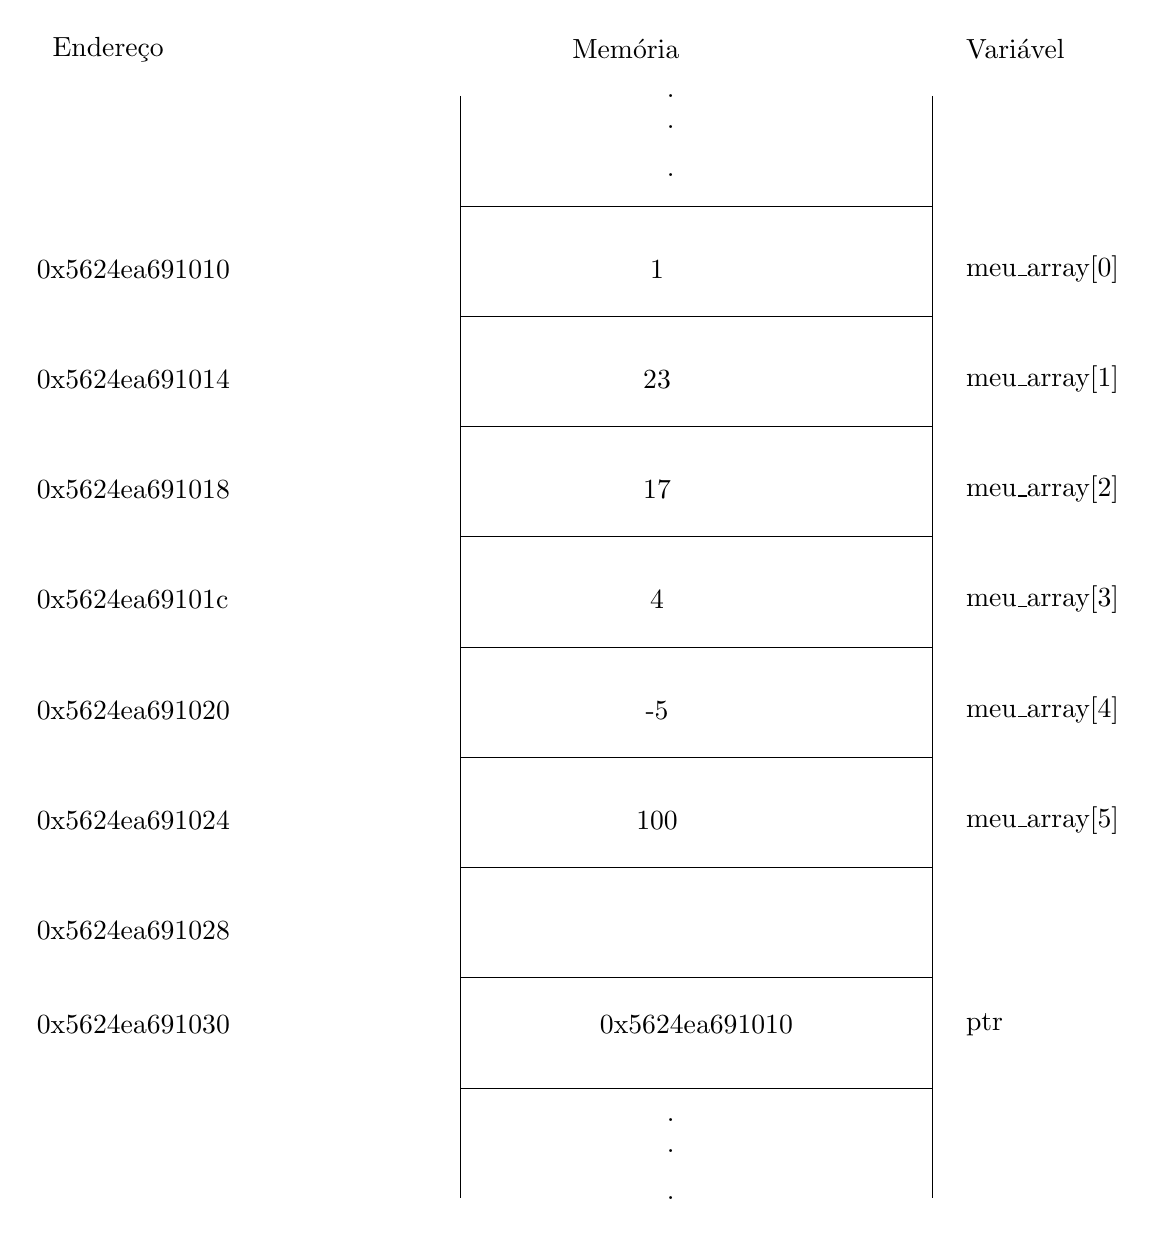
\begin{tikzpicture}
\pgftransformxscale{1.000000}
\pgftransformyscale{-1.000000}
\definecolor{dialinecolor}{rgb}{0.000000, 0.000000, 0.000000}
\pgfsetstrokecolor{dialinecolor}
\definecolor{dialinecolor}{rgb}{1.000000, 1.000000, 1.000000}
\pgfsetfillcolor{dialinecolor}

\draw (31\du,9.4\du)--(31.\du,8\du)--(25\du,8\du)--(25\du,9.4\du);
\node at (27.5\du,8.8\du){1};
\draw (31\du,10.8\du)--(31.\du,9.4\du)--(25\du,9.4\du)--(25\du,10.8\du);
\node at (27.5\du,10.2\du){23};
\draw (31\du,12.2\du)--(31.\du,10.8\du)--(25\du,10.8\du)--(25\du,12.2\du);
\node at (27.5\du,11.6\du){17};
\draw (31\du,13.6\du)--(31.\du,12.2\du)--(25\du,12.2\du)--(25\du,13.6\du);
\node at (27.5\du,13\du){4};
\draw (31\du,15\du)--(31.\du,13.6\du)--(25\du,13.6\du)--(25\du,15\du);
\node at (27.5\du,14.4\du){-5};
\draw (31\du,16.4\du)--(31.\du,15\du)--(25\du,15\du)--(25\du,16.4\du);
\node at (27.5\du,15.8\du){100};
\draw (31\du,17.8\du)--(31.\du,16.4\du)--(25\du,16.4\du)--(25\du,17.8\du);
\node at (28\du,18.4\du){0x5624ea691010};
\draw (31\du,17.8\du)--(31.\du,16.4\du)--(25\du,16.4\du)--(25\du,17.8\du);
%\node at (27.5\du,18.6\du){0110 1100};
\draw (31\du,19.2\du)--(31.\du,17.8\du)--(25\du,17.8\du)--(25\du,19.2\du)--cycle;
\node[anchor=west] at (27.5\du,20.6\du){.};
\node[anchor=west] at (27.5\du,20\du){.};
\node[anchor=west] at (27.5\du,19.6\du){.};

\definecolor{dialinecolor}{rgb}{0.000000, 0.000000, 0.000000}
\pgfsetstrokecolor{dialinecolor}
\draw (25\du,19.2\du)--(25\du,20.6\du);
\draw (31\du,19.2\du)--(31\du,20.6\du);
\draw (25\du,6.6\du)--(25\du,8\du);
\draw (31\du,6.6\du)--(31\du,8\du);
\node[anchor=west] at (27.5\du,7.600000\du){.};
\node[anchor=west] at (27.5\du,7.000000\du){.};
\node[anchor=west] at (27.5\du,6.600000\du){.};
\node[anchor=west] at (19.5\du,8.8\du){0x5624ea691010};
\node[anchor=west] at (19.5\du,10.2\du){0x5624ea691014};
\node[anchor=west] at (19.5\du,11.6\du){0x5624ea691018};
\node[anchor=west] at (19.5\du,13\du){0x5624ea69101c};
\node[anchor=west] at (19.5\du,14.4\du){0x5624ea691020};
\node[anchor=west] at (19.5\du,15.8\du){0x5624ea691024};
\node[anchor=west] at (19.5\du,17.2\du){0x5624ea691028};
\node[anchor=west] at (19.5\du,18.4\du){0x5624ea691030};
\node[anchor=west] at (19.7\du,6.002347\du) {Endere\c{c}o};
\node[anchor=west] at (26.3\du,6.002347\du){Mem\'{o}ria};
\node[anchor=west] at (31.3\du,6.002347\du){Vari\'{a}vel};
\node[anchor=west] at (31.3\du,8.8\du){meu\_array[0]};
\node[anchor=west] at (31.3\du,10.2\du){meu\_array[1]};
\node[anchor=west] at (31.3\du,11.6\du){meu\_array[2]};
\node[anchor=west] at (31.3\du,13\du){meu\_array[3]};
\node[anchor=west] at (31.3\du,14.4\du){meu\_array[4]};
\node[anchor=west] at (31.3\du,15.8\du){meu\_array[5]};
\node[anchor=west] at (31.3\du,18.4\du){ptr};
\end{tikzpicture}

		\caption{Ponteiros e arrays.}
		\label{fig:pontarrays}
	\end{center}
\end{figure}

Anteriormente, ao discutir o termo ``lvalue'', citei K\&R-2, onde afirmava:

\begin{quotation}
	``Um \textbf{objeto} é uma região nomeada de armazenamento; um \textbf{lvalue} é uma expressão que se refere a um objeto''.
\end{quotation}

Isso levanta um problema interessante. Visto que \textbf{meu\_array} é uma região nomeada de armazenamento, por que \textbf{meu\_array} na instrução de atribuição acima não é um \textit{lvalue}? Para resolver esse problema, alguns se referem a \textbf{meu\_array} como um ``\textit{lvalue} não modificável''.

Modifique o programa de exemplo anterior mudando
\begin{lstlisting}
	ptr = &meu_array[0];
\end{lstlisting}
para
\begin{lstlisting}
	ptr = meu_array;
\end{lstlisting}
e execute-o novamente para verificar se os resultados são idênticos.

Agora, vamos nos aprofundar um pouco mais na diferença entre os nomes \textbf{ptr} e \textbf{meu\_array} como usados acima. Alguns escritores se referem ao nome de um array como um ponteiro constante. O que queremos dizer com isso? Bem, para entender o termo ``\textbf{\textit{constante}}'' neste sentido, vamos voltar à nossa definição do termo ``variável''. Quando declaramos uma variável, reservamos um ponto na memória para armazenar o valor do tipo apropriado. Feito isso, o nome da variável pode ser interpretado de duas maneiras. Quando usado no lado esquerdo do operador de atribuição, o compilador o interpreta como o local da memória para o qual mover aquele valor resultante da avaliação do lado direito do operador de atribuição. Mas, quando usado no lado direito do operador de atribuição, o nome de uma variável é interpretado como significando o conteúdo armazenado naquele endereço de memória reservado para conter o valor dessa variável.

Com isso em mente, vamos agora considerar a mais simples das constantes, como em:
\begin{lstlisting}
	int i, k;
	i = 2;
\end{lstlisting}

Aqui, enquanto \textbf{i} é uma variável e então ocupa espaço na porção de dados da memória, 2 é uma constante e, como tal, em vez de reservar memória no segmento de dados, é embutido diretamente no segmento de código da memória. Ou seja, ao escrever algo como \textbf{k = i;} dizemos ao compilador para criar um código que, em tempo de execução, examinará a localização da memória \textbf{\&i} para determinar o valor a ser movido para \textbf{k}, o código criado por \textbf{i = 2;} simplesmente coloca o 2 no código e não há referência ao segmento de dados. Ou seja, \textbf{k} e \textbf{i} são objetos, mas 2 não é um objeto.

Da mesma forma, no exemplo acima, uma vez que \textbf{meu\_array} é uma constante, uma vez que o compilador estabelece onde o próprio \textit{array} deve ser armazenado, ele ``sabe'' o endereço de \textbf{meu\_array[0]} e ao ver:
\begin{lstlisting}
	ptr = meu_array;
\end{lstlisting}
ele simplesmente usa esse endereço como uma constante no segmento de código e não há referência do segmento de dados além disso.

Este pode ser um bom lugar para explicar melhor o uso da expressão \textbf{(void *)} usada no Programa \ref{prog1-1} do Capítulo 1. Como vimos, podemos ter ponteiros de vários tipos. Até agora, discutimos ponteiros para inteiros e ponteiros para caracteres. Nos próximos capítulos, aprenderemos sobre ponteiros para estruturas e até mesmo ponteiros para ponteiros.

Também aprendemos que em diferentes sistemas o tamanho de um ponteiro pode variar. Acontece que também é possível que o tamanho de um ponteiro possa variar dependendo do tipo de dados do objeto para o qual ele aponta. Assim, como acontece com inteiros nos quais você pode ter problemas ao tentar atribuir um inteiro longo a uma variável do tipo inteiro curto, você pode ter problemas ao tentar atribuir os valores de ponteiros de vários tipos a variáveis de ponteiro de outros tipos.

Para minimizar esse problema, C fornece um ponteiro do tipo \textbf{void}. Podemos declarar tal ponteiro escrevendo:
\begin{lstlisting}
	void *vptr;
\end{lstlisting}

Um ponteiro \textbf{void} é uma espécie de ponteiro genérico. Por exemplo, enquanto C não permite a comparação de um ponteiro para um tipo inteiro com um ponteiro para um tipo caractere, por exemplo, qualquer um deles pode ser comparado a um ponteiro \textbf{void}. Claro, como com outras variáveis, os \textit{casts} podem ser usados para converter de um tipo de ponteiro para outro nas circunstâncias adequadas. No Programa \ref{prog1-1} do Capítulo 1, converto os ponteiros para inteiros em ponteiros vazios para torná-los compatíveis com a especificação de conversão \textbf{\%p}. Em capítulos posteriores, outros \textit{casts} serão feitos pelas razões aqui definidas.

Bem, isso é muito material técnico para digerir e não espero que um iniciante entenda tudo isso na primeira leitura. Com o tempo e experimentação, você vai querer voltar e reler os primeiros 2 capítulos. Mas, por enquanto, vamos prosseguir para a relação entre ponteiros, arrays de caracteres e strings.


\chapterimage{brunton-machine.jpg} % Chapter heading image

\chapter{Ponteiros e Strings}
O estudo de strings é útil para vincular ainda mais a relação entre ponteiros e \textit{arrays}. Também torna fácil ilustrar como algumas das funções de string C padrão podem ser implementadas. Finalmente, ilustra como e quando os ponteiros podem e devem ser passados para funções.

Em C, strings são \textit{arrays} de caracteres. Isso não é necessariamente verdade em outras linguagens. Em \textbf{Java}, \textbf{Python}, \textbf{PHP} e várias outras linguagens, uma string tem seu próprio tipo de dados. Mas em C isso não acontece. Em C, uma string é um \textit{array} de caracteres terminado com um caractere binário zero (escrito como `\textbackslash0'). Para começar nossa discussão, escreveremos um código que, embora seja útil para fins ilustrativos, você provavelmente nunca escreveria em um programa real. Considere, por exemplo:
\begin{lstlisting}
	char my_string[40];
	
	my_string[0] = 'T';
	my_string[1] = 'e';
	my_string[2] = 'd':
	my_string[3] = '\0';
\end{lstlisting}

Embora nunca se construísse uma string como essa, o resultado final é uma string no sentido de que é um \textit{array} de caractere\textbf{s terminado com um caractere nulo}. Por definição, em C, uma string é um \textit{array} de caracteres terminado com o caractere nulo. Esteja ciente de que ``nul'' \textbf{não é} o mesmo que ``\textbf{NULL}''. O nulo se refere a um zero conforme definido pela sequência de escape '\textbf{\textbackslash0}'. Ou seja, ocupa um byte de memória. NULL, por outro lado, é o nome da macro usada para inicializar ponteiros nulos. NULL é definido (com \#define) em um arquivo de cabeçalho em seu compilador C, o caractere nulo não pode ser definido por \#define.

Uma vez que escrever o código acima consumiria muito tempo, C permite duas maneiras alternativas de obter a mesma coisa. Primeiro, pode-se escrever:
\begin{lstlisting}
	char my_string[40] = {'T', 'e', 'd', '\0',};
\end{lstlisting}

Mas isso também exige mais digitação do que o conveniente. Então, C permite:
\begin{lstlisting}
	char my_string[40] = "Ted";
\end{lstlisting}

Quando as aspas duplas são usadas, em vez das aspas simples como foi feito nos exemplos anteriores, o caractere nulo ('\textbf{\textbackslash0}') é automaticamente anexado ao final da string.

Em todos os casos acima, acontece a mesma coisa. O compilador separa um bloco contíguo de memória de 40 bytes para conter caracteres e o inicializa de forma que os primeiros 4 caracteres sejam \textbf{Ted\textbackslash0}.

Agora, considere o seguinte programa:
\lstinputlisting[label=prog:strings, caption=Ponteiros e strings, numbers=left]{code/prog3-1.c}

No Programa \ref{prog:strings}, começamos definindo dois \textit{arrays} de caracteres de 80 caracteres cada. Como eles são definidos globalmente, eles são inicializados com todos os '\textbackslash0's primeiro. Então, \textbf{strA} tem os primeiros 36 caracteres inicializados para a string entre aspas (cada caractere acentuado ou cedilha ocupa o espaço de dois caracteres).

Agora, entrando no código, declaramos dois ponteiros de caracteres e mostramos a string na tela. Em seguida, ``apontamos'' o ponteiro \textbf{pA} para \textbf{strA}. Ou seja, por meio da instrução de atribuição, copiamos o endereço de \textbf{strA[0]} em nossa variável \textbf{pA}. Agora usamos \textbf{puts()} para mostrar o que é apontado por \textbf{pA} na tela. Considere aqui que o protótipo de função para \textbf{puts()} é:
\begin{lstlisting}
	int puts(const char *s);
\end{lstlisting}

Por enquanto, ignore o \textbf{const}. O parâmetro passado para \textbf{puts()} é um ponteiro, isto é, o \textbf{valor} de um ponteiro (já que todos os parâmetros em C são passados por valor), e o valor de um ponteiro é o endereço para o qual ele aponta, ou, simplesmente, um endereço . Assim, quando escrevemos \textbf{puts(strA);} como vimos, estamos passando o endereço de \textbf{strA[0]}.

Da mesma forma, quando escrevemos \textbf{puts(pA);} estamos passando o mesmo endereço, pois definimos pA = strA;

Dado isso, siga o código até a instrução \textbf{while()} na linha A. A linha A declara:

\textit{Enquanto o caractere apontado por \textbf{pA} (ou seja, \textbf{*pA}) não for um caractere nulo (ou seja, a terminação `\textbf{\textbackslash0}'), faça a linha B.}

A linha B declara: 

\textit{Copie o caractere apontado por \textbf{pA} para o espaço apontado por \textbf{pB}, então incremente \textbf{pA} de forma que aponte para o próximo caractere e \textbf{pB} para que aponte para o próximo espaço.}

Depois de copiar o último caractere, \textbf{pA} agora aponta para o caractere \textit{nulo} de terminação e o loop termina. No entanto, não copiamos o caractere nulo. E, por definição, uma string em C deve ter terminação nula. Então, adicionamos o caractere nulo com a linha C.

É muito educativo executar este programa com seu \textit{debugger} enquanto acompanha \textbf{strA}, \textbf{strB}, \textbf{pA} e \textbf{pB} e avança passo a passo pelo programa. É ainda mais educacional se, em vez de simplesmente definir \textbf{strB[]} como foi feito acima, inicialize-o também com algo como:

\begin{lstlisting}
	strB[80] = "12345678901234567890123456789012345678901234567890"
\end{lstlisting}
onde o número de dígitos usados é maior do que o comprimento de \textbf{strA} e, em seguida, repita o procedimento de passo único enquanto observa as variáveis acima. Experimente isso!

Voltando ao protótipo de \textbf{puts()} por um momento, o ``\textit{const}'' usado como um modificador de parâmetro informa ao usuário que a função não modificará a string apontada por \textbf{s}, ou seja, ela tratará aquela string como uma constante.

Claro, o que o programa acima ilustra é uma maneira simples de copiar uma string. Depois de brincar com os itens acima até que você tenha uma boa compreensão do que está acontecendo, podemos prosseguir com a criação de nosso próprio substituto para o \textbf{strcpy()} padrão que vem com C. Pode ser parecido com:
\lstinputlisting[label=prog:meustrcpy, caption=Meu strcpy(), numbers=left, lastline=10]{code/prog3-2.c}

Nesse caso, segui a prática usada na rotina padrão de retornar um ponteiro ao destino.

Novamente, a função é projetada para aceitar os valores de dois ponteiros de caracteres, ou seja, endereços e, portanto, no programa anterior, poderíamos escrever:
\lstinputlisting[label=prog:mainmeustrcpy, caption=Main de meu\_strcpy(), numbers=left, firstline=12, lastline=15]{code/prog3-2.c}

Eu me desviei um pouco da forma usada no padrão C, que teria o protótipo:
\begin{lstlisting}
	char *meu_strcpy(char *destino, const char *fonte);
\end{lstlisting}

Aqui, o modificador ``\textit{const}'' é usado para garantir ao usuário que a função não modificará o conteúdo apontado pelo ponteiro de origem. Você pode provar isso modificando a função acima, e seu protótipo, para incluir o modificador ``\textit{const}''  conforme mostrado. Então, dentro da função, você pode adicionar uma instrução que tenta alterar o conteúdo do que é apontado pela fonte, como:
\begin{lstlisting}
	*fonte = 'X';
\end{lstlisting}
que normalmente mudaria o primeiro caractere da string para um X. O modificador \textit{const} deve fazer com que seu compilador pegue isso como um erro. Experimente e veja.

Agora, vamos considerar algumas das coisas que os exemplos acima nos mostraram. Em primeiro lugar, considere o fato de que \textbf{*ptr++} deve ser interpretado como retornando o valor apontado por \textbf{ptr} e, em seguida, incrementando o valor do ponteiro. Isso tem a ver com a precedência dos operadores. Se escrevêssemos \textbf{(*ptr)++}, não incrementaríamos o ponteiro, mas aquilo para o qual o ponteiro aponta! Ou seja, se usado no primeiro caractere da string de exemplo acima, o `T' seria incrementado para um `U'. Você pode escrever alguns códigos simples de exemplo  para ilustrar isso.

Lembre-se novamente de que uma string nada mais é do que um \textit{array} de caracteres, com o último caractere sendo '\textbf{\textbackslash0}'. O que fizemos acima foi lidar com a cópia de um \textit{array}. Acontece que é um \textit{array} de caracteres, mas a técnica poderia ser aplicada a um \textit{array} de inteiros, doubles, etc. Nesses casos, no entanto, não estaríamos lidando com strings e, portanto, o final do \textit{array} não seria marcado com um valor especial como o caractere nulo. Poderíamos implementar uma versão que contasse com um valor especial para identificar o fim. Por exemplo, podemos copiar um \textit{array} de inteiros positivos marcando o final com um inteiro negativo. Por outro lado, é mais comum que, quando escrevemos uma função para copiar um \textit{\textit{array}} de itens que não sejam strings, passemos à função o número de itens a serem copiados, bem como o endereço do \textit{array}, por exemplo, algo como o seguinte protótipo pode indicar:
\begin{lstlisting}
	void int_copy(int *ptrA, int *ptrB, int n);
\end{lstlisting}
onde \textbf{n} é o número de inteiros a serem copiados. Você pode querer brincar com essa ideia e criar um \textit{array} de inteiros e ver se consegue escrever a função \textbf{int\_copy(}) e fazê-la funcionar.

Isso permite o uso de funções para manipular grandes \textit{arrays}. Por exemplo, se temos um \textit{array} de 5000 inteiros que queremos manipular com uma função, precisamos apenas passar para essa função o endereço do \textit{array} (e qualquer informação auxiliar como \textbf{n} acima, dependendo do que estamos fazendo). O \textit{array} em si não é passado, ou seja, o \textit{array} de inteiros não é copiado e colocado na pilha antes de chamar a função, apenas seu endereço é enviado.

Isso é diferente de passar, digamos, um número inteiro para uma função. Quando passamos um inteiro, fazemos uma cópia do inteiro, ou seja, obtemos seu valor e o colocamos na pilha. Dentro da função, qualquer manipulação do valor passado não pode de forma alguma afetar o inteiro original. Mas, com \textit{arrays} e ponteiros, podemos passar o endereço da variável e, portanto, manipular os valores das variáveis originais.


\chapterimage{carbonated-water-device} % Chapter heading image

\chapter{Mais sobre Strings}
Bem, nós progredimos bastante em pouco tempo! Vamos recuar um pouco e ver o que foi feito no Capítulo 3 sobre cópia de strings, mas sob uma luz diferente. Considere a seguinte função:
\lstinputlisting[label=prog:meustrcpy4, caption= meu\_strcpy() com arrays, numbers=left, lastline=11]{code/prog4-1.c}

Lembre-se de que as strings são \textit{arrays} de caracteres. Aqui, escolhemos usar a notação de \textit{array} em vez da notação de ponteiro para fazer a cópia real. Os resultados são os mesmos, ou seja, a string é copiada usando essa notação com a mesma precisão de antes. Isso levanta alguns pontos interessantes que discutiremos.

Como os parâmetros são passados por valor, tanto na passagem de um ponteiro de caractere quanto no nome do \textit{array} como acima, o que realmente é passado é o endereço do primeiro elemento de cada \textit{array}. Assim, o valor numérico do parâmetro passado é o mesmo se usarmos um ponteiro de caractere ou um nome de \textit{array} como parâmetro. Isso tenderia a implicar que de alguma forma \textbf{fonte[i]} é o mesmo que \textbf{*(p + i)}.

De fato, isso é verdade, ou seja, sempre que alguém escreve um \textbf{a[i]}, ele pode ser substituído por \textbf{*(a + i)} sem problemas. Na verdade, o compilador criará o mesmo código em ambos os casos. Portanto, vemos que a aritmética de ponteiro é a mesma coisa que a indexação de \textit{array}. Qualquer sintaxe produz o mesmo resultado.

Isso NÃO quer dizer que ponteiros e \textit{arrays} sejam a mesma coisa, eles não são. Estamos apenas dizendo que, para identificar um determinado elemento de um \textit{array}, temos a opção de duas sintaxes, uma usando indexação de \textit{array} e a outra usando aritmética de ponteiros, que produzem resultados idênticos.

Agora, olhando para esta última expressão, parte dela ... \textbf{(a + i)}, é uma adição simples usando o operador \textbf{+} e as regras de C afirmam que tal expressão é comutativa. Ou seja, \textbf{(a + i)} é idêntico a \textbf{(i + a)}. Assim, poderíamos escrever \textbf{*(i + a)} tão facilmente quanto \textbf{*(a + i)}.

Mas \textbf{*(i + a)} poderia ter vindo de \textbf{i[a]}! De tudo isso vem a curiosa verdade que se:
\begin{lstlisting}
	char a[20];
	int i;
\end{lstlisting}
escrever
\begin{lstlisting}
	a[3] = 'x';
\end{lstlisting}
é o mesmo que escrever
\begin{lstlisting}
	3[a] = 'x'
\end{lstlisting}

Tente! Configure um array de caracteres, inteiros ou longos, etc. e atribua ao terceiro ou quarto elemento um valor usando a abordagem convencional e, em seguida, imprima esse valor para ter certeza de que está funcionando. Em seguida, inverta a notação do \textit{array} como fiz acima. Um bom compilador não hesitará e os resultados serão idênticos. Uma curiosidade ... nada mais!

Agora, olhando para a nossa função, quando escrevemos:
\begin{lstlisting}
	dest[i] = fonte[i];
\end{lstlisting}
devido ao fato de que a indexação de \textit{array} e a aritmética de ponteiro produzem resultados idênticos, podemos escrever isso como:
\begin{lstlisting}
	*(dest + i) = *(fonte + i);
\end{lstlisting}

Mas, isso faz 2 adições para cada valor assumido por i. As adições, em geral, levam mais tempo do que as incrementações (como aquelas feitas usando o operador \textbf{++} como em \textbf{i++}). Isso pode não ser verdade em compiladores de otimização modernos, mas nunca se pode ter certeza. Portanto, a versão do ponteiro pode ser um pouco mais rápida do que a versão do \textit{array}.

Outra forma de acelerar a versão do ponteiro seria alterar:
\begin{lstlisting}
	while (*fonte != '\0')
\end{lstlisting}
para simplesmente
\begin{lstlisting}
	while (*fonte)
\end{lstlisting}
já que o valor entre parênteses irá para zero (FALSO) ao mesmo tempo em ambos os casos.

Neste ponto, você pode querer experimentar um pouco escrevendo alguns de seus próprios programas usando ponteiros. Manipulação strings é um bom lugar para experimentar. Você pode querer escrever suas próprias versões de funções padrão como:
\begin{lstlisting}
	strlen();
	strcat();
	strchr();
\end{lstlisting}
e quaisquer outras que você possa ter em seu sistema.

Voltaremos às strings e sua manipulação por meio de ponteiros em um capítulo futuro. Por enquanto, vamos prosseguir e discutir um pouco as estruturas.


\chapterimage{metal-turning-lathe} % Chapter heading image

\chapter{Ponteiros e Estruturas}
Como você deve saber, podemos declarar um bloco de dados contendo diferentes tipos de dados por meio de uma declaração de estrutura. Por exemplo, um arquivo de pessoal pode conter estruturas que se parecem com:
\begin{lstlisting}
	struct tag {
		char sobrenome[20];
		char nome[20];
		int idade;
		float salario;
	};
\end{lstlisting}

Digamos que temos várias dessas estruturas em um arquivo em disco, e queremos ler e imprimir o nome e o sobrenome de cada registro para que possamos ter uma lista das pessoas em nossos arquivos. As informações restantes não serão impressas. Queremos fazer essa impressão com uma chamada de função e passar para essa função um ponteiro para a estrutura em questão. Para fins de demonstração, usarei apenas uma estrutura por enquanto. Mas perceba que o objetivo é a escrita da função, não a leitura do arquivo que, presumivelmente, sabemos fazer.

Para revisão, lembre-se de que podemos acessar membros da estrutura com o operador ponto como em:
\lstinputlisting[label={prog5-1}, caption={Estruturas}, numbers=left, numberstyle=\tiny, stepnumber=1]{code/prog5-1.c}

Agora, esta estrutura em particular é bem pequena comparada àquelas normalmente usadas em programas C. À estrutura acima, podemos adicionar:
\begin{lstlisting}
	data_de_admissao;
	data_do_ultimo_aumento;
	ultimo_percentual_de_aumento;
	telefone_de_emergencia;
	plano_de_saude;
	numero_de_previdencia;
	etc.....
\end{lstlisting}

Se temos um grande número de funcionários, o que queremos fazer é manipular os dados dessas estruturas por meio de funções. Por exemplo, podemos querer que uma função imprima o nome do funcionário listado em qualquer estrutura passada a ela. Porém, no C original (\textit{Kernighan \& Ritchie}, 1ª Edição) não era possível passar uma estrutura, apenas um ponteiro para uma estrutura poderia ser passado. Desde \textbf{ANSI C}, é permitido passar a estrutura completa. Mas, como nosso objetivo aqui é aprender mais sobre ponteiros, não vamos nos estender nisso.

De qualquer forma, se passarmos a estrutura inteira, isso significa que devemos copiar o conteúdo da estrutura da função que chama para a função que é chamada. Em sistemas que usam pilhas, isso é feito fazendo um \textit{push} do conteúdo da estrutura para a pilha. Com grandes estruturas, isso pode ser um problema. No entanto, passar um ponteiro usa uma quantidade mínima de espaço de pilha.

Em qualquer caso, como esta é uma discussão sobre ponteiros, discutiremos como passamos um ponteiro para uma estrutura e então o usamos dentro da função.

Considere o caso descrito, ou seja, queremos uma função que aceite como parâmetro um ponteiro para uma estrutura e de dentro dessa função queremos acessar os membros da estrutura. Por exemplo, queremos imprimir o nome do funcionário em nossa estrutura de exemplo.

Ok, então sabemos que nosso ponteiro irá apontar para uma estrutura declarada usando a \textit{struct tag}. Declaramos tal ponteiro com a declaração:
\begin{lstlisting}
	(*st_ptr).idade = 63;
\end{lstlisting}

Olhe com atenção. Ele diz: substitua o que está entre parênteses pelo que \textbf{st\_ptr} aponta, que é a estrutura \textbf{minha\_struct}. Portanto, é o mesmo que \textbf{minha\_struct.idade}.

No entanto, esta é uma expressão usada com bastante frequência e os designers de C criaram uma sintaxe alternativa com o mesmo significado, que é:
\begin{lstlisting}
	st_ptr->idade = 63;
\end{lstlisting}

Com isso em mente, observe o seguinte programa:
\lstinputlisting[label={prog5-2}, caption={Ponteiros e Estruturas}, numbers=left, numberstyle=\tiny, stepnumber=1]{code/prog5-2.c}

Novamente, essa é uma grande quantidade de informações para absorver de uma vez. O leitor deve compilar e executar os vários trechos de código e usar um depurador para monitorar coisas como \textbf{minha\_struct} e \textbf{p} enquanto percorre o \textbf{main} e segue o código para dentro da função para ver o que está acontecendo.
\chapterimage{printing-form} % Chapter heading image

\chapter{Mais sobre Strings e Arrays de Strings}
Bem, vamos voltar um pouco às strings. A seguir, todas as atribuições devem ser entendidas como globais, ou seja, feitas fora de qualquer função, incluindo \textit{main()}.

Indicamos em um capítulo anterior que poderíamos escrever:
\begin{lstlisting}
	char minha_string[40] = "Ted";
\end{lstlisting}
que alocaria espaço para um \textit{array} de 40 bytes e colocaria a string nos primeiros 4 bytes (três para os caracteres entre aspas e um quarto para lidar com a terminação '\textbf{\textbackslash0}').

Na verdade, se tudo o que quiséssemos fazer fosse armazenar o nome ``Ted'', poderíamos escrever:
\begin{lstlisting}
	char meu_nome[] = "Ted";
\end{lstlisting}
e o compilador contaria os caracteres, deixaria espaço para o caractere nulo e armazenaria o total dos quatro caracteres na memória, cuja localização seria retornada pelo nome do \textit{array}, neste caso \textbf{meu\_nome}.

Em algum código, em vez do descrito acima, você verá:
\begin{lstlisting}
	char *meu_nome = "Ted";
\end{lstlisting}
que é uma abordagem alternativa. Existe alguma diferença entre eles? A resposta é... sim. Usando a notação de \textit{array}, 4 bytes de armazenamento no bloco de memória estática são ocupados, um para cada caractere e um para o caractere nulo de terminação. Mas, na notação de ponteiro, os mesmos 4 bytes necessários, mais \textbf{N} bytes para armazenar a variável de ponteiro \textbf{meu\_nome} (onde \textbf{N} depende do sistema, mas geralmente tem um mínimo de 2 bytes e pode ser 4 ou mais). Veja a Figura \ref{fig:arrayponteiro}.

\begin{figure}[ht]
	\begin{center}
		% Graphic for TeX using PGF
% Title: /home/araujo/Dropbox/VerbTeX/LivroComputadores/Pictures/memoria.dia
% Creator: Dia v0.97.3
% CreationDate: Sun May 21 11:59:17 2017
% For: araujo
% \usepackage{tikz}
% The following commands are not supported in PSTricks at present
% We define them conditionally, so when they are implemented,
% this pgf file will use them.
\ifx\du\undefined
  \newlength{\du}
\fi
\setlength{\du}{15\unitlength}

\begin{tikzpicture}
\pgftransformxscale{1.000000}
\pgftransformyscale{-1.000000}
\definecolor{dialinecolor}{rgb}{0.000000, 0.000000, 0.000000}
\pgfsetstrokecolor{dialinecolor}
\definecolor{dialinecolor}{rgb}{1.000000, 1.000000, 1.000000}
\pgfsetfillcolor{dialinecolor}

%cabeçalho
\node[anchor=west] at (21.3\du,7.5\du) {Endere\c{c}o};
\node[anchor=west] at (24.4\du,6.002347\du){Mem\'{o}ria};
\node[anchor=west] at (27.3\du,7.5\du){Array};

%conteúdo
\node[anchor=west] at (25.6\du,6.600000\du){.};
\node[anchor=west] at (25.6\du,7.000000\du){.};
\node[anchor=west] at (25.6\du,7.600000\du){.};
\node at (26\du,8.8\du) {'T'};
\node at (26\du,10.2\du){'e'};
\node at (26\du,11.6\du){'d'};
\node at (26\du,13\du)  {'\textbackslash0'};
\node[anchor=west] at (25.6\du,19.6\du){.};
\node[anchor=west] at (25.6\du,20\du){.};
\node[anchor=west] at (25.6\du,20.6\du){.};

%retângulos
\draw (25\du,6.6\du)--(25\du,8.0\du)--(27\du,8\du)--(27\du,6.6\du);
\draw (25\du,8.0\du)--(25\du,9.4\du)--(27\du,9.4\du)--(27\du,8\du);
\draw (25\du,9.4\du)--(25\du,10.8\du)--(27\du,10.8\du)--(27.\du,9.4\du);
\draw (25\du,10.8\du)--(25\du,12.2\du)--(27\du,12.2\du)--(27.\du,10.8\du);
\draw (25\du,12.2\du)--(25\du,13.6\du)--(27\du,13.6\du)--(27.\du,12.2\du);
\draw (25\du,13.6\du)--(25\du,15\du)--(27\du,15\du)--(27.\du,13.6\du);
\draw (25\du,15\du)--(25\du,16.4\du)--(27\du,16.4\du)--(27.\du,15\du);
\draw (25\du,16.4\du)--(25\du,17.8\du)--(27\du,17.8\du)--(27.\du,16.4\du);
\draw (25\du,17.8\du)--(25\du,19.2\du)--(27\du,19.2\du)--(27.\du,17.8\du);
\draw (25\du,19.2\du)--(25\du,20.6\du);
\draw (27\du,19.2\du)--(27\du,20.6\du);

%endereços
\node[anchor=west] at (21\du,8.8\du) {0x5a691010};
\node[anchor=west] at (21\du,10.2\du){0x5a691011};
\node[anchor=west] at (21\du,11.6\du){0x5a691012};
\node[anchor=west] at (21\du,13\du)  {0x5a691013};
\node[anchor=west] at (21\du,14.4\du){0x5a691014};
\node[anchor=west] at (21\du,15.8\du){0x5a691015};
\node[anchor=west] at (21\du,17.2\du){0x5a691016};
\node[anchor=west] at (21\du,18.4\du){0x5a691017};

% variáveis
\node[anchor=west] at (27.3\du,8.8\du){meu\_array};

%ponteiro
%cabeçalho
\node[anchor=west] at (33.3\du,7.5\du) {Endere\c{c}o};
\node[anchor=west] at (36.4\du,6.002347\du){Mem\'{o}ria};
\node[anchor=west] at (39.3\du,7.57\du){Ponteiro};

%conteúdo
\node[anchor=west] at (37.6\du,6.600000\du){.};
\node[anchor=west] at (37.6\du,7.000000\du){.};
\node[anchor=west] at (37.6\du,7.600000\du){.};
\node at (38\du,8.8\du) {'T'};
\node at (38\du,10.2\du){'e'};
\node at (38\du,11.6\du){'d'};
\node at (38\du,13\du)  {'\textbackslash0'};
\node at (38\du,14.4\du) {10};
\node at (38\du,15.8\du) {10};
\node at (38\du,17.2\du) {69};
\node at (38\du,18.6\du) {5a};
\node[anchor=west] at (37.6\du,19.6\du){.};
\node[anchor=west] at (37.6\du,20\du){.};
\node[anchor=west] at (37.6\du,20.6\du){.};

%retângulos
\draw (37\du,6.6\du)--(37\du,8.0\du)--(39\du,8\du)--(39\du,6.6\du);
\draw (37\du,8.0\du)--(37\du,9.4\du)--(39\du,9.4\du)--(39\du,8\du);
\draw (37\du,9.4\du)--(37\du,10.8\du)--(39\du,10.8\du)--(39.\du,9.4\du);
\draw (37\du,10.8\du)--(37\du,12.2\du)--(39\du,12.2\du)--(39.\du,10.8\du);
\draw (37\du,12.2\du)--(37\du,13.6\du)--(39\du,13.6\du)--(39.\du,12.2\du);
\draw (37\du,13.6\du)--(37\du,15\du)--(39\du,15\du)--(39.\du,13.6\du);
\draw (37\du,15\du)--(37\du,16.4\du)--(39\du,16.4\du)--(39.\du,15\du);
\draw (37\du,16.4\du)--(37\du,17.8\du)--(39\du,17.8\du)--(39.\du,16.4\du);
\draw (37\du,17.8\du)--(37\du,19.2\du)--(39\du,19.2\du)--(39.\du,17.8\du);
\draw (37\du,19.2\du)--(37\du,20.6\du);
\draw (39\du,19.2\du)--(39\du,20.6\du);

%endereços
\node[anchor=west] at (33\du,8.8\du) {0x5a691010};
\node[anchor=west] at (33\du,10.2\du){0x5a691011};
\node[anchor=west] at (33\du,11.6\du){0x5a691012};
\node[anchor=west] at (33\du,13\du)  {0x5a691013};
\node[anchor=west] at (33\du,14.4\du){0x5a691014};
\node[anchor=west] at (33\du,15.8\du){0x5a691015};
\node[anchor=west] at (33\du,17.2\du){0x5a691016};
\node[anchor=west] at (33\du,18.4\du){0x5a691017};

% variáveis
\node[anchor=west] at (39.3\du,8.8\du){*meu\_array};
\node[anchor=west] at (39.4\du,16.4\du){meu\_array};

\draw [decorate, ultra thick,
decoration = {calligraphic brace}] (39.3\du,13.6\du) --  (39.3\du,19.2\du);

\end{tikzpicture}

		\caption{Uso da memória com Array e Ponteiro (cada posição 1 byte).}
		\label{fig:arrayponteiro}
	\end{center}
	\label{enderecos}
\end{figure}

Na notação de \textit{array}, \textbf{meu\_nome} é a abreviação de \textbf{\&meu\_nome[0]}, que é o endereço do primeiro elemento do \textit{array}. Como a localização do \textit{array} é fixada durante o tempo de execução, isso é uma constante (não uma variável). Na notação de ponteiro, \textbf{meu\_nome} é uma variável. Quanto a qual é o \textbf{melhor} método, isso depende do que você vai fazer no resto do programa.

Vamos agora dar um passo adiante e considerar o que acontece se cada uma dessas declarações for feita dentro de uma função, em oposição a globalmente fora dos limites de qualquer função.

\begin{lstlisting}
	void minha_funcao_A(char *ptr)
		{
		char a[] = "ABCDE";
		.
		.
		}
		
	void minha_funcao_B(char *ptr)
		{
		char *cp = "FGHIJ";
		.
		.
		}
\end{lstlisting}

No caso de \textbf{minha\_funcao\_A}, o conteúdo, ou valor(es) do \textit{array} \textbf{a[]} é considerado como sendo os dados. Diz-se que o \textit{array} foi inicializado com os valores \textbf{ABCDE}. No caso de \textbf{minha\_funcao\_B}, o valor do ponteiro \textbf{cp} é considerado como sendo o dado. O ponteiro foi inicializado para apontar para a string \textbf{FGHIJ}. Tanto em \textbf{minha\_funcao\_A} quanto em \textbf{minha\_funcao\_B} as definições são variáveis locais e, portanto, a string \textbf{ABCDE} é armazenada na pilha, assim como o valor do ponteiro \textbf{cp}. A string \textbf{FGHIJ} pode ser armazenada em qualquer lugar. No meu sistema, ele fica armazenado no segmento de dados, também conhecido como \textit{heap}. Nas Figuras \ref{fig:memarray} e \ref{fig:mempointer} podemos ver como esses elementos são alocados na pilha (stack) ou na memória de dados (heap) conforme a forma de sua declaração.

\begin{figure}[ht]
	\begin{center}
		\includegraphics[width=0.5\textwidth]{Pictures/memarray}
		\caption{Declaração de string com Array.}
		\label{fig:memarray}
	\end{center}
\end{figure}

\begin{figure}[ht]
	\begin{center}
		\includegraphics[width=0.5\textwidth]{Pictures/mempointer}
		\caption{Declaração de string com Ponteiro.}
		\label{fig:mempointer}
	\end{center}
\end{figure}

A propósito, a inicialização do \textit{array} de variáveis automáticas como fiz em \textbf{minha\_funcao\_A} era ilegal no livro \textit{K\&R} C antigo e apenas ``atingiu a maioridade'' a partir do ANSI C. Um fato que pode ser importante quando se considera portabilidade e compatibilidade com versões anteriores.

Já que estamos discutindo o relacionamento/diferenças entre ponteiros e \textit{arrays}, vamos prosseguir para os \textit{arrays} multidimensionais. Considere, por exemplo, o \textit{array}:
\begin{lstlisting}
	char multi[5][10];
\end{lstlisting}

O que isso significa? Bem, vamos considerar uma declaração com a seguinte configuração:\\  	char \underline{multi[5]}[10];

Vamos considerar a parte sublinhada como o ``nome'' de um \textit{array}. Depois, acrescentando \textbf{char} e o \textbf{[10]}, temos um \textit{array} de 10 caracteres. Mas, o próprio nome \textbf{multi[5]} é um \textit{array} que indica que existem 5 elementos, cada um sendo um \textit{array} de 10 caracteres. Portanto, temos um \textit{array} de 5 \textit{arrays} de 10 caracteres cada.

Suponha que preenchemos este \textit{array} bidimensional com algum tipo de dado. Na memória, pode parecer que foi formado pela inicialização de 5 \textit{arrays} separados usando algo como:
\begin{lstlisting}
	multi[0] = {'0','1','2','3','4','5','6','7','8','9'}
	multi[1] = {'a','b','c','d','e','f','g','h','i','j'}
	multi[2] = {'A','B','C','D','E','F','G','H','I','J'}
	multi[3] = {'9','8','7','6','5','4','3','2','1','0'}
	multi[4] = {'J','I','H','G','F','E','D','C','B','A'}
\end{lstlisting}

Ao mesmo tempo, elementos individuais podem ser endereçados usando uma sintaxe como:
\begin{lstlisting}
	multi[0][3] = '3'
	multi[1][7] = 'h'
	multi[4][0] = 'J'
\end{lstlisting}

Como os \textit{arrays} são contíguos na memória, nosso bloco de memória real para o caso acima deve ser semelhante a:

\vspace{1em}
\ifx\du\undefined
\newlength{\du}
\fi
\setlength{\du}{15\unitlength}
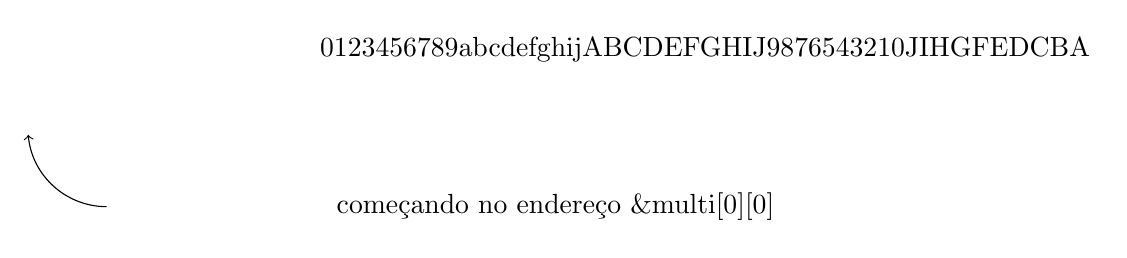
\begin{tikzpicture}
\pgftransformxscale{1.000000}
\pgftransformyscale{-1.000000}
\definecolor{dialinecolor}{rgb}{0.000000, 0.000000, 0.000000}
\pgfsetstrokecolor{dialinecolor}
\definecolor{dialinecolor}{rgb}{1.000000, 1.000000, 1.000000}
\pgfsetfillcolor{dialinecolor}

\node at (3\du,0\du){0123456789abcdefghijABCDEFGHIJ9876543210JIHGFEDCBA};
\draw[->] (-4.6\du, 2\du) arc (90:175:1);
\node at (1.1\du, 2\du){começando no endereço \&multi[0][0]};
\end{tikzpicture}

Observe que eu não escrevi \textbf{multi[0] = "0123456789"}. Se eu tivesse feito isso, uma terminação `\textbf{\textbackslash0}' estaria implícita, pois sempre que as aspas duplas são usadas, um caractere `\textbf{\textbackslash0}' é anexado aos caracteres contidos nessas aspas. Se fosse esse o caso, eu teria que reservar um espaço para 11 caracteres por linha em vez de 10.

Meu objetivo aqui é ilustrar como a memória é configurada para \textit{arrays} bidimensionais. Ou seja, este é um \textit{array} bidimensional de caracteres, NÃO um \textit{array} de ``strings''.

Agora, o compilador sabe quantas colunas estão presentes no \textit{array} para que possa interpretar \textbf{multi + 1} como o endereço do `a' na 2ª linha. Ou seja, ele adiciona 10, o número de colunas, para obter essa localização. Se estivéssemos lidando com inteiros e um \textit{array} com a mesma dimensão, o compilador adicionaria \textbf{10 * sizeof(int)} que, na minha máquina, seria 40.
Assim, o endereço do 9 na 4ª linha acima seria \&multi[3][0] ou *(multi + 3) em notação de ponteiros. Para obter o conteúdo do 2º elemento na 4ª linha, adicionamos 1 a este endereço e desreferenciamos o resultado como em
\begin{lstlisting}
	*(*(multi + 3) + 1)
\end{lstlisting}

Com um pouco de reflexão, podemos ver que:
\begin{lstlisting}
	*(*(multi + row) + col) e
	multi[row][col] levam aos mesmo resultado.
\end{lstlisting}

O programa a seguir ilustra isso usando \textit{arrays} de inteiros em vez de \textit{arrays} de caracteres.

\lstinputlisting[label={prog6-1}, caption={Array bidimensional e ponteiros}, numbers=left, numberstyle=\tiny, stepnumber=1]{code/prog6-1.c}

Por causa da dupla desreferência necessária na versão do ponteiro, o nome de um \textit{array} bidimensional é frequentemente considerado equivalente a um ponteiro para um ponteiro. Com um \textit{array} tridimensional estaríamos lidando com um \textit{array} de \textit{arrays} de \textit{arrays} e alguns podem dizer que seu nome seria equivalente a um ponteiro para um ponteiro para um ponteiro. No entanto, aqui inicialmente reservamos o bloco de memória para o \textit{array}, definindo-o usando a notação de \textit{array}. Portanto, estamos lidando com uma constante, não uma variável. Ou seja, estamos falando de um endereço fixo, não de um ponteiro variável. A função de desreferenciação usada acima nos permite acessar qualquer elemento no \textit{array} de \textit{arrays} sem a necessidade de alterar o valor desse endereço (o endereço de \textbf{multi[0][0]} conforme fornecido pelo símbolo \textbf{multi}).

\chapterimage{beating-washing-engines} % Chapter heading image

\chapter{Mais sobre Arrays Multidimensionais}
No capítulo anterior, notamos que dado
\begin{lstlisting}
	#define LINHAS 5
	#define COLUNAS 10
	
	int multi[LINHAS][COLUNAS];
\end{lstlisting}
podemos acessar elementos individuais do \textit{array} \textbf{multi} usando:
\begin{lstlisting}
	multi[lin][col]
\end{lstlisting}
ou
\begin{lstlisting}
	*(*(multi + lin) + col)
\end{lstlisting}

Para entender mais completamente o que está acontecendo, vamos substituir
\begin{lstlisting}
	*(multi + lin)
\end{lstlisting}
por \textbf{X}, como em:
\begin{lstlisting}
	*(X + col)
\end{lstlisting}

Agora, a partir disso, vemos que \textbf{X} é como um ponteiro, já que a expressão é desreferenciada e sabemos que \textbf{col} é um inteiro. Aqui, a aritmética usada é de um tipo especial chamado ``aritmética de ponteiro''. Isso significa que, como estamos falando de um \textit{array} de inteiros, o endereço apontado por (ou seja, valor de) \textbf{X + col + 1} deve ser maior do que o endereço \textbf{X + col} por uma quantidade igual a \textbf{sizeof(int)}.

Uma vez que conhecemos o layout da memória para \textit{arrays} bidimensionais, podemos determinar que na expressão \textbf{multi + lin} como usada acima, \textbf{multi + lin + 1} deve aumentar por valor um valor igual ao necessário para ``apontar para'' a próxima linha, que neste caso, seria um valor igual a \textbf{COLUNAS * sizeof(int)}.

Isso significa que se a expressão \textbf{*(*(multi + lin) + col)} deve ser avaliada corretamente em tempo de execução, o compilador deve gerar o código que leva em consideração o valor de \textbf{COLUNAS}, ou seja, a 2ª dimensão. Por causa da equivalência das duas formas de expressão, isso é verdade quer estejamos usando a expressão de ponteiro como aqui ou a expressão de \textit{array} \textbf{multi[linha][col]}.

Assim, para avaliar qualquer uma das expressões, um total de 5 valores deve ser conhecido:
\begin{enumerate}
	\item O endereço do primeiro elemento do array, que é retornado pela expressão \textbf{multi}, ou seja, o nome do \textbf{array}.
	\item O tamanho do tipo dos elementos do \textit{array}, neste caso \textbf{sizeof(int)}.
	\item A 2ª dimensão do \textit{array}.
	\item O valor de índice específico para a primeira dimensão, \textbf{lin} neste caso.
	\item O valor de índice específico para a segunda dimensão, \textbf{col} neste caso.
\end{enumerate}

Dado tudo isso, considere o problema de projetar uma função para manipular os valores dos elementos de um \textit{array} previamente declarado. Por exemplo, um que definiria todos os elementos do \textit{array} \textbf{multi} para o valor 1.

\begin{lstlisting}
	void define_valor(int m_array[][COLUNAS])	{
		for (int lin = 0; lin < LINHAS; lin++){
			for (int col = 0; col < COLUNAS; col++){
				m_array[lin][col] = 1;
			}
		}
	}
\end{lstlisting}

E para chamar essa função, usaríamos:
\begin{lstlisting}
	define_valor(multi);
\end{lstlisting}

Agora, dentro da função, usamos os valores \textit{\#defined} por LINHAS e COLUNAS que definem os limites dos \textit{loops} \textbf{for}. Mas, esses \textit{\#defines} são apenas constantes no que diz respeito ao compilador, ou seja, não há nada que os conecte ao tamanho do \textit{array} dentro da função. \textbf{lin} e \textbf{col} são variáveis locais, é claro. A definição formal do parâmetro permite ao compilador determinar as   características associadas ao valor do ponteiro que será passado em tempo de execução. Realmente não precisamos da primeira dimensão e, como será visto mais tarde, há ocasiões em que preferiríamos não defini-la dentro da definição do parâmetro, por hábito ou consistência, não a usei aqui. Mas, a segunda dimensão deve ser usada como foi mostrado na expressão do parâmetro. A razão é que precisamos disso na avaliação de \textbf{m\_array[lin][col]} como foi descrito. Enquanto o parâmetro define o tipo de dados (\textbf{int} neste caso) e as variáveis automáticas para linha e coluna são definidas nos \textit{loops for}, apenas um valor pode ser passado usando um único parâmetro. Nesse caso, esse é o valor de \textbf{multi} conforme observado na instrução de chamada, ou seja, o endereço do primeiro elemento, muitas vezes referido como um ponteiro para o \textit{array}. Assim, a única forma que temos de informar o compilador da 2ª dimensão é incluindo explicitamente na definição dos parâmetros.

Na verdade, em geral, todas as dimensões de ordem superior à primeira são necessárias ao lidar com \textit{arrays} multidimensionais. Ou seja, se estamos falando de \textit{arrays} tridimensionais, a 2ª e a 3ª dimensões devem ser especificadas na definição do parâmetro.
\chapterimage{scott-printing-press} % Chapter heading image

\chapter{Ponteiros para Arrays}
Os ponteiros, é claro, podem ser ``apontados para'' qualquer tipo de objeto de dados, incluindo \textit{arrays}. Embora isso tenha ficado evidente quando discutimos o Programa \ref{prog:strings}, é importante expandir como fazemos isso quando se trata de \textit{arrays} multidimensionais.

Para revisar, no Capítulo 2, afirmamos que, dado um \textit{array} de inteiros, poderíamos apontar um ponteiro de inteiro para esse \textit{array} usando:
\begin{lstlisting}
	int *ptr;
	ptr = &meu_array[0]; // Aponta nosso ponteiro para o 
	                     // primeiro inteiro de nosso array
\end{lstlisting}

Como afirmamos lá, o tipo da variável de ponteiro deve corresponder ao tipo do primeiro elemento do \textit{array}.

Além disso, podemos usar um ponteiro como um parâmetro formal de uma função projetada para manipular um \textit{array}. por exemplo.

Dado:
\begin{lstlisting}
	int array[3] = {'1', '5', '7'};
	void uma_func(int *p);
\end{lstlisting}

Alguns programadores podem preferir escrever o protótipo da função como:
\begin{lstlisting}
	void uma_func(int p[]);
\end{lstlisting}
que tenderia a informar outras pessoas que poderiam usar esta função que a função foi projetada para manipular os elementos de um \textit{array}. Obviamente, em ambos os casos, o que realmente é passado é o valor de um ponteiro para o primeiro elemento do \textit{array}, independente de qual notação é usada no protótipo ou definição da função. Observe que, se a notação de \textit{array} for usada, não há necessidade de passar a dimensão real do \textit{array}, pois não estamos passando o \textit{array} inteiro, apenas o endereço do primeiro elemento.

Agora nos voltamos para o problema do \textit{array} bidimensional. Conforme declarado no último capítulo, C interpreta um \textit{array} bidimensional como um \textit{array} de \textit{arrays} unidimensionais. Sendo esse o caso, o primeiro elemento de um \textit{array} bidimensional de inteiros é um \textit{array} unidimensional de inteiros. E um ponteiro para um \textit{array} bidimensional de inteiros deve ser um ponteiro para esse tipo de dados. Uma forma de o conseguir é através da utilização da palavra-chave ``\textbf{typedef}''. \textbf{typedef} atribui um novo nome a um tipo de dados especificado. Por exemplo:
\begin{lstlisting}
	typedef unsigned char byte;
\end{lstlisting}
faz com que o nome \textbf{byte} signifique o tipo \textbf{unsigned char}. Portanto
\begin{lstlisting}
	byte b[10];
\end{lstlisting}
seria um \textit{array} de caracteres sem sinal.

Observe que na declaração de \textbf{typedef}, a palavra \textit{byte} substituiu o que normalmente seria o nome de nosso \textbf{unsigned char}. Ou seja, a regra para usar \textbf{typedef} é que o novo nome para o tipo de dados seja o nome usado na definição do tipo de dados. Assim em:
\begin{lstlisting}
	typedef int Array[10];
\end{lstlisting}
\textbf{Array} se torna um tipo de dados para um \textit{array} de 10 inteiros. ou seja, \textbf{Array meu\_arr;} declara \textbf{meu\_arr} como um \textit{array} de 10 inteiros e \textbf{Array arr2d[5];} torna \textbf{arr2d} um \textit{array} de 5 \textit{arrays} de 10 inteiros cada.

Observe também que \textbf{Array *p1d;} torna \textbf{p1d} um ponteiro para um \textit{array} de 10 inteiros. Como \textbf{*p1d} aponta para o mesmo tipo que \textbf{arr2d}, atribuir o endereço do \textit{array} bidimensional \textbf{arr2d} a \textbf{p1d}, o ponteiro para um \textit{array} unidimensional de 10 inteiros é aceitável. ou seja, 
\begin{lstlisting}
	p1d = &arr2d[0];
\end{lstlisting}
ou
\begin{lstlisting}
	p1d = arr2d;
\end{lstlisting}
estão ambos corretos.

Como o tipo de dados que usamos para nosso ponteiro é um \textit{array} de 10 inteiros, esperaríamos que incrementar \textbf{p1d} em 1 mudaria seu valor em \textbf{10 * sizeof(int)}, o que realmente acontece. Ou seja, \textbf{sizeof(*p1d)} é 40 (em um computador com  inteiros de 4 bytes). Você pode provar isso para si mesmo escrevendo e executando um programa curto simples.

Agora, embora o uso de \textbf{typedef} torne as coisas mais claras para o leitor e mais fáceis para o programador, não é realmente necessário. O que precisamos é uma maneira de declarar um ponteiro como \textbf{p1d} sem a necessidade da palavra-chave \textbf{typedef}. Acontece que isso pode ser feito e que
\begin{lstlisting}
	int (*p1d)[10];
\end{lstlisting}
é a declaração apropriada, ou seja, \textbf{p1d} aqui é um ponteiro para um \textit{array} de 10 inteiros, exatamente como estava na declaração usando o tipo \textbf{Array}. Observe que isso é diferente de
\begin{lstlisting}
	int *p1d[10];
\end{lstlisting}
o que tornaria \textbf{p1d} o nome de um \textit{array} de 10 ponteiros para o tipo \textbf{int}.
\chapterimage{oilseed-mill} % Chapter heading image

\chapter{Ponteiros e Alocação Dinâmica de Memória}
Há momentos em que é conveniente alocar memória em tempo de execução usando \textbf{malloc()}, \textbf{calloc()} ou outras funções de alocação. O uso dessa abordagem permite adiar a decisão sobre o tamanho do bloco de memória necessário para armazenar um \textit{array}, por exemplo, até o tempo de execução. Ou permite usar uma seção de memória para o armazenamento de um \textit{array} de inteiros em um ponto no tempo, e então quando essa memória não for mais necessária, ela pode ser liberada para outros usos, como o armazenamento de um \textit{array} de estruturas.

Quando a memória é alocada, a função de alocação (como \textbf{malloc()}, \textbf{calloc()}, etc.) retorna um ponteiro. O tipo deste ponteiro depende se você está usando um compilador \textbf{K\&R} mais antigo ou o compilador mais recente. Com o compilador mais antigo, o tipo do ponteiro retornado é \textbf{char}, com compiladores atuais é \textbf{void}.

Se você estiver usando um compilador mais antigo e quiser alocar memória para um \textit{array} de inteiros, terá que converter o ponteiro \textbf{char} retornado para um ponteiro inteiro. Por exemplo, para alocar espaço para 10 inteiros, podemos escrever:
\begin{lstlisting}
	int *iptr;
	iptr = (int *)malloc(10 * sizeof(int));
	if (iptr == NULL)
	{ .. A ROTINA DE ERROS VAI AQUI .. }
\end{lstlisting}

Se você estiver usando um compilador atual, \textbf{malloc()} retorna um ponteiro \textbf{void} e como um ponteiro \textbf{void} pode ser atribuído a uma variável de ponteiro de qualquer tipo de objeto, o \textit{cast} \textbf{(int *)} mostrado acima não é necessário: 
\begin{lstlisting}
	int *iptr;
	iptr = malloc(10 * sizeof(int));
\end{lstlisting}
A dimensão do \textit{array} pode ser determinada em tempo de execução e não é necessária em tempo de compilação. Ou seja, o 10 acima pode ser uma variável lida de um arquivo de dados ou teclado, ou calculada com base em alguma necessidade, em tempo de execução.

Por causa da equivalência entre a notação de \textit{array} e ponteiro, uma vez que \textbf{iptr} tenha sido atribuído como acima, pode-se usar a notação de \textit{array}. Por exemplo, pode-se escrever:
\begin{lstlisting}
	int k;
	for (k = 0; k < 10; k++)
		iptr[k] = 2;
\end{lstlisting}
para definir os valores de todos os elementos para 2.

Mesmo com um entendimento razoavelmente bom de ponteiros e \textit{arrays}, um lugar que o novato em C provavelmente tropeçará no início é na alocação dinâmica de \textit{arrays} multidimensionais. Em geral, gostaríamos de poder acessar elementos de tais \textit{arrays} usando notação de \textit{array}, não notação de ponteiro, sempre que possível. Dependendo da aplicação, podemos ou não saber as duas dimensões no momento da compilação. Isso nos leva a diversas maneiras de realizar nossa tarefa.

Como vimos, ao alocar dinamicamente um \textit{array} unidimensional, sua dimensão pode ser determinada em tempo de execução. Agora, ao usar a alocação dinâmica de \textit{arrays} de ordem superior, nunca precisamos saber a primeira dimensão em tempo de compilação. Se precisamos saber as dimensões superiores depende de como vamos escrever o código. Aqui, discutirei vários métodos de alocação dinâmica de espaço para \textit{arrays} bidimensionais de inteiros.

\section*{MÉTODO 1:}
Uma maneira de lidar com o problema é usando a palavra-chave \textbf{typedef}. Para alocar um \textit{array} bidimensional de inteiros, lembre-se de que as duas notações a seguir resultam na geração do mesmo código de objeto:
\begin{lstlisting}
	multi[lin][col] = 1;         // Usando array
	*(*(multi + lin) + col) = 1; // Usando ponteiro
\end{lstlisting}

Também é verdade que as duas notações a seguir geram o mesmo código:
\begin{lstlisting}
	multi[lin];     // Usando array
	*(multi + lin); // Usando ponteiro
\end{lstlisting}

Visto que a segunda linha deve ser avaliada como um ponteiro, a notação de \textit{array} da primeira linha também deve ser avaliada como um ponteiro. Na realidade, \textbf{multi[0]} retornará um ponteiro para o primeiro inteiro na primeira linha, \textbf{multi[1]} um ponteiro para o primeiro inteiro da segunda linha, etc. Na verdade, \textbf{multi[n]} avalia como um ponteiro para aquele \textit{array} de inteiros que constituem a enésima linha de nosso array bidimensional. Ou seja, \textbf{multi} pode ser pensado como um \textit{array} de \textit{arrays} e \textbf{multi[n]} como um ponteiro para o enésimo \textit{array} deste \textit{array} de \textit{arrays}. Aqui, a palavra ponteiro está sendo usada para representar um valor de endereço. Embora tal uso seja comum na literatura, ao ler tais declarações deve-se ter o cuidado de distinguir entre o endereço constante de um \textit{array} e um ponteiro de variável, que é um objeto de dados em si.

Considere agora:
\lstinputlisting[label=prog:ponteiros, caption=Ponteiros e malloc, numbers=left]{code/prog9-1.c}

Aqui, assumi um compilador atual, portanto, uma conversão no ponteiro \textbf{void} retornado por \textbf{malloc()} não é necessária. Se você estivesse usando um compilador \textbf{K\&R }mais antigo, teria que converter usando:
\begin{lstlisting}
	lptr = (ArrayLinha *)malloc(nlinhas * COLS * sizeof(int));
\end{lstlisting}

Usando esta abordagem, \textbf{lptr} tem todas as características de um nome de \textit{array}, (exceto que \textbf{lptr} é modificável), e a notação de \textit{array} pode ser usada em todo o resto do programa. Isso também significa que, se você pretende escrever uma função para modificar o conteúdo do \textit{array}, deve usar \textbf{COLS} como parte do parâmetro formal dessa função, assim como fizemos ao discutir a passagem de \textit{arrays} bidimensionais para uma função.

\section*{MÉTODO 2:}
No MÉTODO 1, \textbf{lptr} acabou sendo um ponteiro para tipo ``um array unidimensional de COLS inteiros''. Acontece que existe uma sintaxe que pode ser usada para esse tipo sem a necessidade de \textbf{typedef}. Se escrevermos:
\begin{lstlisting}
	int (*xptr)[COLS];
\end{lstlisting}
a variável \textbf{xptr} terá todas as características da variável \textbf{lptr} no \textbf{MÉTODO 1}, e não precisamos usar a palavra-chave \textit{typedef}. Aqui \textbf{xptr} é um ponteiro para um \textit{array} de inteiros e o tamanho desse \textit{array} é dado por \textbf{\#define COLS}. O posicionamento dos parênteses faz com que a notação de ponteiro predomine, embora a notação de \textit{array} tenha precedência mais alta. ou seja, se houvéssemos escrito
\begin{lstlisting}
	int *xptr[COLS];
\end{lstlisting}
teríamos definido \textbf{xptr} como um \textit{array} de ponteiros contendo o número de ponteiros igual ao \textbf{\#definido} por \textbf{COLS}. Isso não é a mesma coisa de forma alguma. No entanto, \textit{arrays} de ponteiros têm seu uso na alocação dinâmica de \textit{arrays} bidimensionais, como será visto nos próximos 2 métodos.

\section*{MÉTODO 3:}
Considere o caso em que não sabemos o número de elementos em cada linha em tempo de compilação, ou seja, o número de linhas e o número de colunas devem ser determinados em tempo de execução. Uma maneira de fazer isso seria criar um \textit{array} de ponteiros para o tipo \textbf{int} e então alocar espaço para cada linha e apontar esses ponteiros para cada linha. Considere:
\lstinputlisting[label=prog:metodo3, caption=Método 3, numbers=left]{code/prog9-2.c}

No código anterior, \textbf{ptrlinha} é um ponteiro de um ponteiro para o tipo \textbf{int}. Nesse caso, ele aponta para o primeiro elemento de um \textit{array} de ponteiros para o tipo \textbf{int}. Considere o número de chamadas para \textbf{malloc()}:

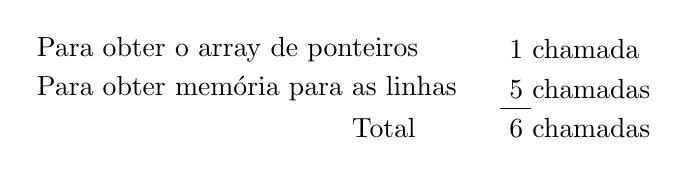
\begin{tikzpicture}
\node[anchor=west] at (0,0)    {Para obter o array de ponteiros};
\node[anchor=west] at (0,-0.5) {Para obter memória para as linhas};
\node[anchor=west] at (4,-1) {Total};
\node[anchor=west] at (6,0)    {1 chamada};
\node[anchor=west] at (6,-0.5) {5 chamadas};
\node[anchor=west] at (6,-1) {6 chamadas};
\draw (6,-0.75) -- (6.4,-0.75);
\end{tikzpicture}

Se você optar por usar esta abordagem, observe que, embora você possa usar a notação de \textit{array} para acessar elementos individuais do \textit{array}, por exemplo, \textbf{ptrlinha[lin][col] = 42;}, isso não significa que os dados no ``\textit{array} bidimensional'' são contíguos na memória.

Você pode, entretanto, usar a notação de \textit{array} como se fosse um bloco contínuo de memória. Por exemplo, você pode escrever:
\begin{lstlisting}
	ptrlinha[lin][col] = 176;
\end{lstlisting}
exatamente como se \textbf{ptrlinha} fosse o nome de um \textit{array} bidimensional criado em tempo de compilação. É claro que \textbf{lin} e \textbf{col} devem estar dentro dos limites do \textit{array} que você criou, assim como com um \textit{array} criado em tempo de compilação.

Se você deseja ter um bloco contíguo de memória dedicado ao armazenamento dos elementos do \textit{array}, pode fazê-lo da seguinte maneira:

\section*{MÉTODO 4:}
Neste método, alocamos um bloco de memória para armazenar primeiro o \textit{array} inteiro. Em seguida, criamos um \textit{array} de ponteiros para apontar para cada linha. Portanto, mesmo que o \textit{array} de ponteiros esteja sendo usado, o \textit{array} real na memória é contíguo. O código é parecido com este:
\lstinputlisting[label=prog:metodo4, caption=Método 4., numbers=left]{code/prog9-3.c}

Considere novamente, o número de chamadas para \textbf{malloc()}

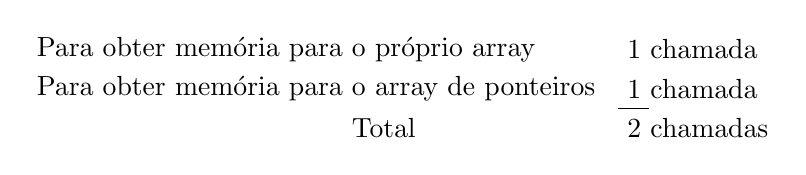
\begin{tikzpicture}
\node[anchor=west] at (0,0)    {Para obter memória para o próprio array};
\node[anchor=west] at (0,-0.5) {Para obter memória para o array de ponteiros};
\node[anchor=west] at (4,-1) {Total};
\node[anchor=west] at (7.5,0)    {1 chamada};
\node[anchor=west] at (7.5,-0.5) {1 chamada};
\node[anchor=west] at (7.5,-1) {2 chamadas};
\draw (7.5,-0.75) -- (7.9,-0.75);
\end{tikzpicture}

Agora, cada chamada para \textbf{malloc()} cria uma sobrecarga de espaço adicional, já que \textbf{malloc()} é geralmente implementado pelo sistema operacional formando uma lista encadeada que contém dados relativos ao tamanho do bloco. Mas, mais importante, com grandes arrays (várias centenas de linhas), controlar o que precisa ser liberado quando chega a hora pode ser mais complicado. Isso, combinado com a contiguidade do bloco de dados que permite a inicialização para todos os zeros usando \textbf{memset()}, parece tornar a segunda alternativa a preferida.

Como um exemplo final em \textit{arrays} multidimensionais, ilustraremos a alocação dinâmica de um \textit{array} tridimensional. Este exemplo ilustrará mais uma coisa a se observar ao fazer esse tipo de alocação. Pelas razões citadas anteriormente, usaremos a abordagem descrita na alternativa dois. Considere o seguinte código:
\lstinputlisting[label=prog:tridimensional, caption=Alocação de Array Tridimensional.., numbers=left]{code/prog9-4.c}

Se você seguiu este tutorial até este ponto, não deverá ter problemas para decifrar o programa \ref{prog:tridimensional} com base apenas nos comentários. No entanto, há alguns pontos que devem ser destacados. Vamos começar com a linha que diz:
\begin{lstlisting}
	Arr3D[z][y] = espaco + (z * (X_DIM * Y_DIM) + y * X_DIM);
\end{lstlisting}

Observe que aqui \textbf{espaço} é um ponteiro de caractere, que é do mesmo tipo que \textbf{Arr3D[z][y]}. É importante que ao adicionar um inteiro, como o obtido pela avaliação da expressão \textbf{(z * (X\_DIM * Y\_DIM) + y * X\_DIM)}, a um ponteiro, o resultado seja um novo valor do ponteiro. E ao atribuir valores de ponteiro a variáveis de ponteiro, os tipos de dados do valor e da variável devem corresponder.

\chapterimage{marinoni-printing-press1} % Chapter heading image

\chapter{Ponteiros para Funções}
Até este ponto, discutimos ponteiros para objetos de dados. C também permite a declaração de ponteiros para funções. Os ponteiros para funções têm diversos usos e alguns deles serão discutidos aqui.

Considere o seguinte problema real. Você deseja escrever uma função que seja capaz de ordenar virtualmente qualquer coleção de dados que possa ser armazenada em um \textit{array}. Isso pode ser um \textit{array} de strings, inteiros, pontos flutuantes, ou mesmo estruturas. O algoritmo de classificação pode ser o mesmo para todos. Por exemplo, pode ser um algoritmo de classificação de bolha simples, ou algoritmos mais complexos como o \textit{shellsort} ou o \textit{quicksort}. Usaremos uma ordenação pelo método da bolha simples, para fins de demonstração.

Sedgewick \cite{sedgewick} descreveu a classificação por bolhas usando código C, configurando uma função que, quando passada por um ponteiro para o \textit{array}, iria ordená-lo. Se chamarmos essa função \textbf{bubble()}, um programa de classificação é descrito por \textbf{bubble\_1.c}, que se segue:
\lstinputlisting[label=prog:bubble1, caption=bubble\_1.c, numbers=left]{code/bubble_1.c}

A ordenação pelo método da bolha é um dos tipos mais simples. O algoritmo varre o \textit{array} do segundo ao último elemento, comparando cada elemento com o que o precede. Se aquele que o precede for maior que o elemento atual, os dois serão trocados de forma que o maior fique mais próximo do final do \textit{array}. Na primeira passagem, isso resulta no maior elemento terminando no final do \textit{array}. O \textit{array} agora está limitado a todos os elementos, exceto o último e o processo repetido. Isso coloca o próximo maior elemento em um ponto que precede o maior elemento. O processo é repetido por um número de vezes igual ao número de elementos menos 1. O resultado final é um \textit{array} ordenado.

Aqui, nossa função é projetada para classificar um \textit{array} de inteiros. Portanto, na linha 27 estamos comparando inteiros e nas linhas 28 a 30 estamos usando armazenamento temporário de inteiros para armazenar inteiros. O que queremos fazer agora é ver se podemos converter esse código para que possamos usar qualquer tipo de dados, ou seja, não ficar restrito a inteiros.

Ao mesmo tempo, não queremos ter que analisar nosso algoritmo e o código associado a ele cada vez que o usarmos. Começamos removendo a comparação de dentro da função \textbf{bubble()} para tornar relativamente fácil modificar a função de comparação sem ter que reescrever partes relacionadas ao algoritmo real. Isso resulta em\textbf{ bubble\_2.c} (Programa \ref{prog:bubble2}):
\lstinputlisting[label=prog:bubble2, caption=bubble\_2.c, numbers=left]{code/bubble_2.c}

Se nosso objetivo é tornar nossa função de ordenação independente do tipo de dados, uma maneira de fazer isso é usar ponteiros para o tipo \textit{void} para apontar para os dados em vez de usar o tipo de dados inteiro. Para começar nessa direção, vamos modificar algumas coisas para que os ponteiros possam ser usados. Para começar, usaremos ponteiros para o tipo inteiro (Programa \ref{prog:bubble3}).

\lstinputlisting[label=prog:bubble3, caption=bubble\_3.c, numbers=left]{code/bubble_3.c}

Observe as mudanças. Agora estamos passando um ponteiro para um inteiro (ou array de inteiros) para \textbf{bubble()}. E de dentro de \textit{bubble} estamos passando ponteiros para os elementos do array que queremos comparar com nossa função de comparação. E, é claro, estamos desreferenciando esses ponteiros em nossa função \textbf{compare()} para fazer a comparação real. Nossa próxima etapa será converter os ponteiros em \textbf{bubble()} em ponteiros para o tipo \textit{void}, de modo que a função se torne mais insensível ao tipo. Isso é mostrado em bubble\_4 (Programa \ref{prog:bubble4}).

\lstinputlisting[label=prog:bubble4, caption=bubble\_4.c, numbers=left]{code/bubble_4.c}

Observe que, ao fazer isso, em \textbf{compare()} tivemos que introduzir a conversão dos tipos de ponteiro \textit{void} passados para o tipo real que está sendo classificado. Mas, como veremos mais tarde, está tudo bem. E como o que está sendo passado para \textbf{bubble()} ainda é um ponteiro para um \textit{array} de inteiros, tivemos que converter esses ponteiros para ponteiros nulos quando os passamos como parâmetros em nossa chamada para \textbf{compare()}.

Agora abordamos o problema do que passamos para \textbf{bubble()}. Queremos tornar o primeiro parâmetro dessa função um ponteiro \textit{void} também. Mas, isso significa que dentro de \textbf{bubble()} precisamos fazer algo sobre a variável \textbf{t}, que atualmente é um inteiro. Além disso, onde usamos \textbf{t = p [j-1];} o tipo de \textbf{p[j-1]} precisa ser conhecido para saber quantos bytes copiar para a variável \textbf{t} (ou o que quer que substituamos \textbf{t}).

Atualmente, em \textbf{bubble\_4.c}, o conhecimento em \textbf{bubble()} quanto ao tipo de dados sendo classificados (e, portanto, o tamanho de cada elemento individual) é obtido do fato de que o primeiro parâmetro é um ponteiro para o tipo inteiro. Se quisermos usar \textbf{bubble()} para classificar qualquer tipo de dados, precisamos fazer desse ponteiro um ponteiro para o tipo \textit{void}. Mas, ao fazer isso, perderemos informações sobre o tamanho dos elementos individuais dentro do \textit{array}. Portanto, em \textbf{bubble\_5.c} adicionaremos um parâmetro separado para lidar com essas informações de tamanho.

Essas mudanças, de \textbf{bubble\_4.c} para \textbf{bubble\_5.c} (Programa \ref{prog:bubble5}), são, talvez, um pouco mais extensas do que as que fizemos no passado. Portanto, compare os dois módulos cuidadosamente para verificar as diferenças.

\lstinputlisting[label=prog:bubble5, caption=bubble\_5.c, numbers=left]{code/bubble_5.c}

Observe que alterei o tipo de dados do \textit{array} de \textbf{int} para \textbf{long} para ilustrar as alterações necessárias na função \textbf{compare()}. Em \textbf{bubble()}, eliminei a variável \textbf{t} (que teríamos que mudar do tipo \textit{int} para o tipo \textit{long}). Eu adicionei um \textit{buffer} de tamanho 8 caracteres não sinalizados, que é o tamanho necessário para conter um \textit{long} (isso mudará novamente em futuras atualizações neste código). O ponteiro de caracteres não sinalizados \textbf{*bp} é usado para apontar para a base do \textit{array} a ser ordenado, ou seja, para o primeiro elemento desse \textit{array}.

Também tivemos que modificar o que passamos para \textbf{compare()} e como fazemos a troca de elementos que a comparação indica que precisam ser trocados. O uso de \textbf{memcpy()} e notação de ponteiro em vez de notação de array contribui para essa redução na sensibilidade do tipo.

Novamente, fazer uma comparação cuidadosa de \textbf{bubble\_5.c} com \textbf{bubble\_4.c} pode resultar em uma melhor compreensão do que está acontecendo e por quê.

Vamos agora para \textbf{bubble\_6.c} (Programa \ref{prog:bubble6}), onde usamos a mesma função \textbf{bubble()} que usamos em \textbf{bubble\_5.c} para classificar strings em vez de inteiros longos. É claro que temos que mudar a função de comparação, pois o meio pelo qual as strings são comparadas é diferente daquele pelo qual inteiros longos são comparados. E, em \textbf{bubble\_6.c}, excluímos as linhas dentro de \textbf{bubble()} que foram comentadas em \textbf{bubble\_5.c}.

\lstinputlisting[label=prog:bubble6, caption=bubble\_6.c, numbers=left]{code/bubble_6.c}

Mas, o fato de \textbf{bubble()} não ter sido alterado em relação ao usado em \textbf{bubble\_5.c} indica que essa função é capaz de classificar uma ampla variedade de tipos de dados. O que falta fazer é passar para \textbf{bubble()} o nome da função de comparação que queremos usar para que possa ser verdadeiramente universal. Assim como o nome de um \textit{array} é o endereço do primeiro elemento do \textit{array} no segmento de dados, o nome de uma função indica o endereço dessa função no segmento de código. Portanto, precisamos usar um ponteiro para uma função. Neste caso, a função de comparação.

Os ponteiros para funções devem corresponder às funções apontadas no número e nos tipos dos parâmetros e no tipo do valor de retorno. Em nosso caso, declaramos nosso ponteiro de função como:
\begin{lstlisting}
	int (*fptr)(const void *p1, const void *p2);
\end{lstlisting}

Observe que se tivéssemos escrito:
\begin{lstlisting}
	int *fptr(const void *p1, const void *p2)
\end{lstlisting}
teríamos um protótipo de função para uma função que retornasse um ponteiro para o tipo \textbf{int}. Isso ocorre porque em C o operador parênteses () tem uma precedência mais alta do que o operador ponteiro *. Colocando o parêntese ao redor da string \textbf{(* fptr)}, indicamos que estamos declarando um ponteiro de função.

Agora modificamos nossa declaração de \textbf{bubble()} adicionando, como seu quarto parâmetro, um ponteiro de função do tipo apropriado. Seu protótipo de função torna-se:
\begin{lstlisting}
	void bubble(void *p, int tamanho, int n, 
		          int(*fptr)(const void *, const void *));
\end{lstlisting}

Quando chamamos \textbf{bubble()}, inserimos o nome da função de comparação que queremos usar. \textbf{bubble\_7.c} (Programa \ref{prog:bubble7})  ilustra como essa abordagem permite o uso da mesma função \textbf{bubble()} para classificar diferentes tipos de dados.

\lstinputlisting[label=prog:bubble7, caption=bubble\_7.c, numbers=left]{code/bubble_7.c}
\chapterimage{edisons-electric-pen-1600.jpg} % Chapter heading image

\chapter*{Epílogo}
Escrevi este material em português a partir do excelente material fornecido por Ted Jensen. Tentei contactar Ted pelos endereços fornecidos, mas todas as tentativas foram infrutíferas. Pelos meus cálculos, Ted deve estar com mais de 80 anos no momento que faço esta tradução/atualização/adaptação. Espero que esteja bem, apenas afastado da Internet.

Espero que este material em português seja útil para muitos estudantes e professores, e reforçando meu pedido, se este material foi útil para você, me envia uma mensagem, uma crítica, um elogio, uma correção necessária. É sempre bom saber que outros reconhecem nosso trabalho. 

\section*{Pague-me um café}
Não é necessário nenhum pagamento por este trabalho. Um email é suficiente, mas é claro, se você quer contribuir financeiramente para que eu faça mais livros como este, aceito contribuições por \textbf{PIX}, com a vantagem que você pode enviar mensagem pelo próprio PIX. Minha chave é meu email:\\
\texttt{araujo@eng.uerj.br} 

\begin{flushright}
	João Araujo\\
Outubro de 2021
\end{flushright}



%------------------------------------------------

%----------------------------------------------------------------------------------------
%	BIBLIOGRAPHY
%----------------------------------------------------------------------------------------

\chapter*{Bibliografia}
\addcontentsline{toc}{chapter}{\textcolor{black}{Bibliografia}} % Add a Bibliography heading to the table of contents

\printbibliography[heading=bibempty,type=book]


\end{document}
